
\documentclass[review,3p,times,authoryear,12pt]{elsarticle}

\usepackage{subfigure}
\usepackage{amsmath, amsthm, amssymb}

\usepackage{graphicx}
\usepackage{algorithm}
\usepackage{algorithmic}
\usepackage{clrscode3e}
\usepackage{url}
\usepackage{multirow}
\usepackage{longtable}
\usepackage{color}


\journal{TBD}
\newtheorem{corollary}{Corollary}
\newtheorem{theorem}{Theorem}
\newtheorem{definition}{Definition}
\newtheorem{proposition}{Proposition}
\newtheorem{lemma}{Lemma}
\begin{document}
\graphicspath{{./figure/}}
\begin{frontmatter}
\newpage

\title{Target guided algorithms for the container pre-marshalling problem}

\author{Ning Wang}
\ead{wangning@cityu.edu.hk}

\author{Bo Jin\corref{corl}}
\ead{msjinbo@cityu.edu.hk}

\author{Andrew Lim}
\ead{lim.andrew@cityu.edu.hk}

\address{
Department of Management Sciences, City University of Hong Kong, 83 Tat Chee Ave, Kowloon Tong, Hong Kong
}
\cortext[corl]{Corresponding author. Tel: +852 34425296}

\begin{abstract}
Container pre-marshalling problem (CPMP) aims to rearrange containers in a bay with the least movement effort; thus, in the final layout, containers are piled according to a predetermined order. Previous researchers, without exception, assumed that all the stacks in a bay are functionally identical. Such a classical problem setting is reexamined in this paper. Moreover, a new problem, that is, CPMP with a Dummy Stack~(CPMPDS), is proposed.
At terminals with transfer lanes, a bay includes a row of ordinary stacks and a dummy stack. The dummy stack is actually the bay space that is reserved for trucks. Therefore, containers can be shipped out of the bay. During the pre-marshalling process, the dummy stack temporarily stores containers as an ordinary stack.
However, the dummy stack must be emptied at the end of pre-marshalling. In this paper, target-guided algorithms are proposed to handle both classical CPMP and new CPMPDS. All proposed algorithms guarantee termination. Improved lower bounds of CPMP and CPMPDS are also devised. Experimental results in terms of CPMP show that the proposed algorithms surpass the state-of-the-art algorithm.
\end{abstract}

\begin{keyword}
container pre-marshalling \sep target-guided algorithms\sep lower bound \sep dummy stack
\end{keyword}
\end{frontmatter}

\section{Introduction}

Seaborne transportation is the cornerstone of international trade and undoubtedly an engine of global economic development. According to the \textit{Review of Maritime Transport}~(2012) released by united nations conference on trade and development, approximately 80\% of global trade by volume is carried by sea. Among different ship types, container ships account for approximately 62\% of dry cargoes. Since the commencement of containerization, containers facilitate smooth flow of goods across multiple transportation modes without direct freight handling during the course of shipping. Accompany with the rapid growth of container shipping, container terminals face unprecedented development opportunities.
The role of container terminals lies in providing physical spaces for container exchanges between sea and land. At terminals, a large proportion of land spaces (known as container yards or warehouses) are reserved for storing containers temporarily. A yard acts as a cache that ensures rapid loading and unloading of vessels. Basically, a conventional practice of exporting containers is to store them on the yard first. When vessels arrive, containers are transported by trucks to the quayside and then loaded onto vessels. The process is reverse for importing containers.

High efficiency is a key factor for any successful terminal because shipping line managers prefer efficient terminals. Carriers or shippers bear the pressure of quick delivery from downstream customers. Moreover, high efficiency increases the turnover rate of terminals and therefore generates more profit for shareholders. Container terminals have every reason to increase their operational efficiency. Terminal practitioners and OR researchers have paid considerable attention to improving the efficiency of quayside operations. Nonetheless, overall terminal productivity will not increase dramatically if only quayside operations are optimized, thereby leaving yard operations inefficient~\citep{Jiang2012}.

A yard is generally divided into several blocks. A block is composed of several parallel bays. Each bay is formed by several stacks aligned side by side. In each stack, containers are piled vertically. Figure \ref{fig:1} shows a diagram of a yard. The height of stacks is constrained by the height of operating equipment. One stack can typically store 3 to 10 containers.

\begin{figure}[htbp]
\centering
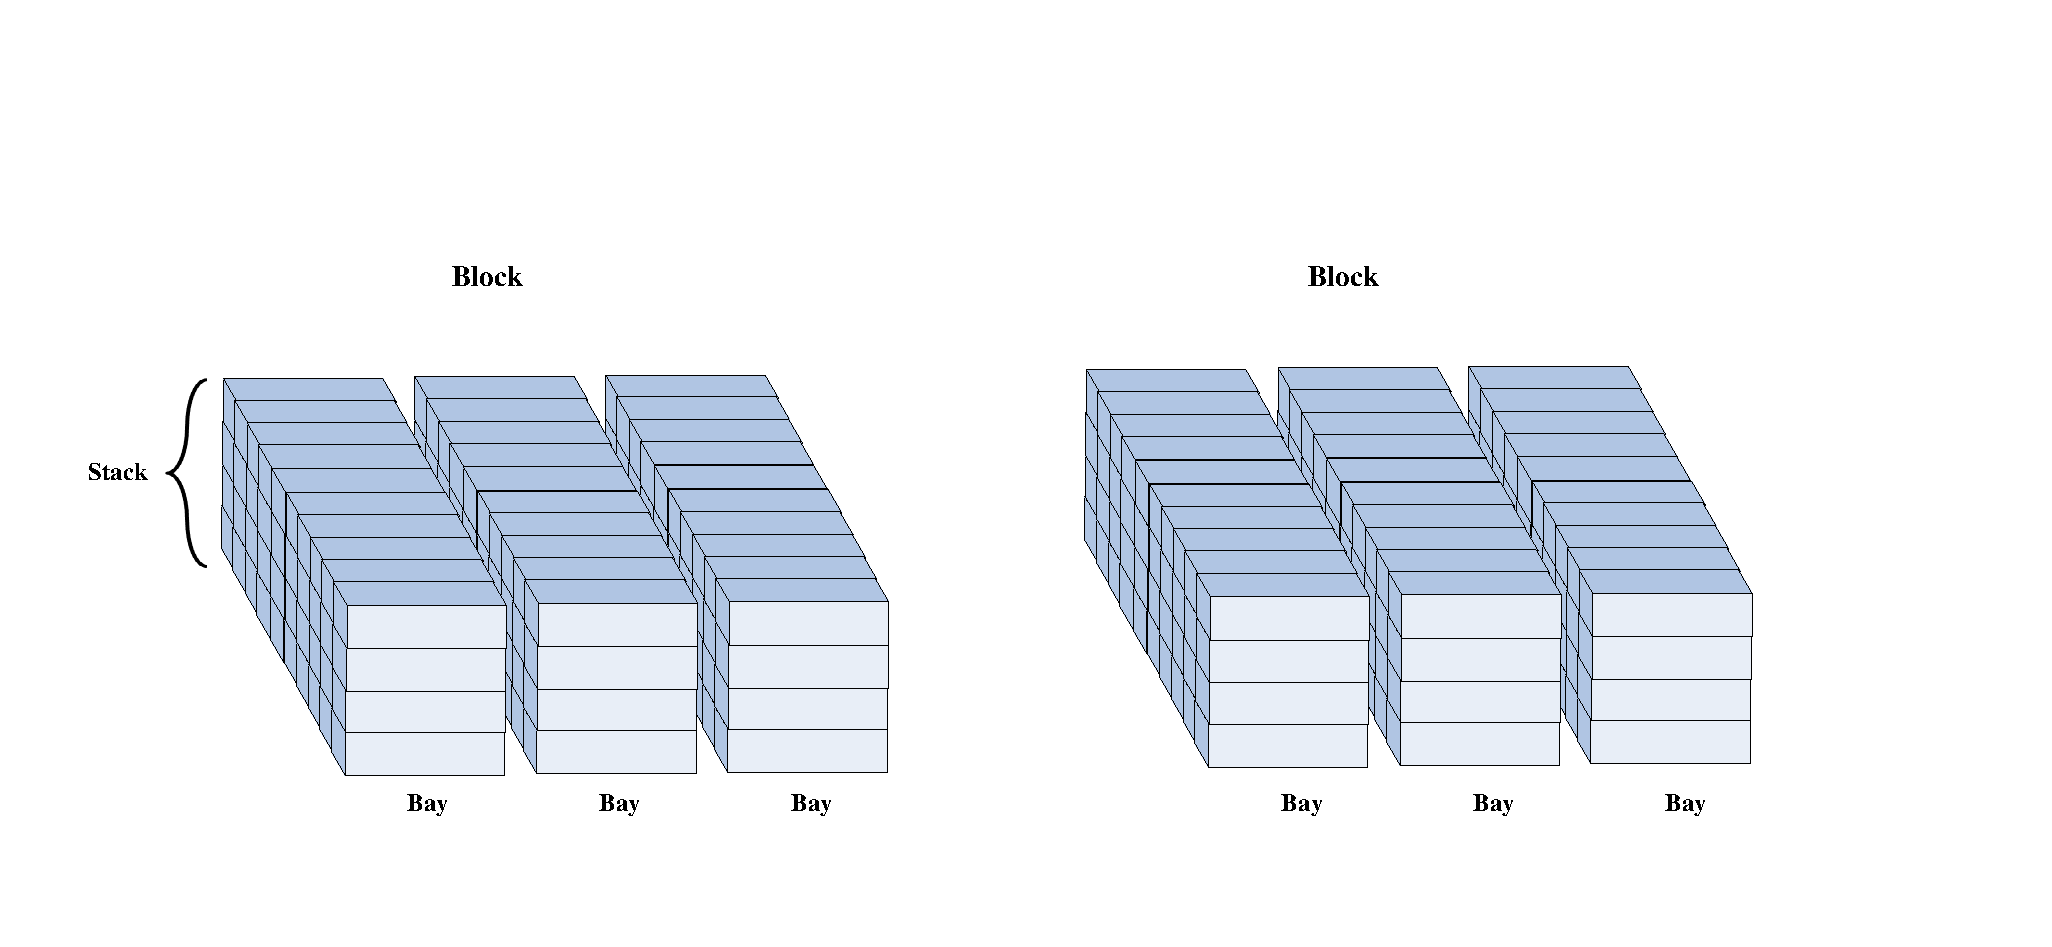
\includegraphics[width=0.60\textwidth]{fig1.pdf}
\caption{An example of a container yard}
\label{fig:1}
\end{figure}

Containers in the same stack can only be retrieved in a ``first in-last out'' manner. If the container to be fetched is not at the top of a stack, all the containers placed above it have to be relocated to other stacks before retrieving it. Such forced movements are known as rehandles. Container Rehandle is costly because this additional task decreases the efficiency of container retrieval, but consignors do not pay for this task. In the ideal situation, containers are piled in an order that is consistent with the retrieval order, i.e., containers retrieved earlier are located at higher tiers. However, the actual situation is the opposite. The placement order of containers is decided by inland transportation or consignors, whereas the retrieval order of containers is decided by stowage planning or ship schedules. In most situations, the two orders are not exactly reverse. In reality, containers that arrive early do not necessarily depart late.

Prior to ship arrival, containers in a bay can be rearranged to comply with their retrieval order. This process is called pre-marshalling. Although it is not billable to consignors, pre-marshalling can reduce berthing time of ships and increase terminal turnover rate. Performing container pre-marshalling with the least effort is denoted as CPMP.
%In the CPMP, a set of containers piled in a bay are given, and each container is assigned with a group label which represents its retrieval batch ordinal. A movement can only move a container from the top of a stack to the top of another stack, resulting in a new layout. The objective of the CPMP is to find the shortest movement sequence which rearranges containers and pile them according to the descending order of group labels from the bottom up.

%One conventional objective is to minimize the number of movements. Gantry movement is a reasonable indicator, as gantry cranes can only process $20 \scriptsize{\sim} 25$ container movements per hour \cite{Rotter2004}, which suggests that gantry cranes are definitely a kind of valuable resource.


Although CPMP has been studied, practical scenarios have not been fully depicted. For terminals that use gantry cranes, there exist two kinds of layouts of I/O points where trucks and gantry cranes exchange containers~\cite{Carlo2014}. Figure \ref{fig15} show the difference of two layouts. In the first layout, I/O points form lanes~(transfer lane) which are parallel to a block while in the second layout, I/O points form bays which are at both ends of a block. In the first layout, when no container is being retrieved, transfer lanes act as temporary stacks for the pre-marshalling work as ordinary stacks. The only issue that demands attention is that transfer lanes should be empty again after the pre-marshalling work, which distinguishes themselves from ordinary stacks. Transfer lanes are called \textbf{dummy stacks}.
%If regarding the extra space as a dummy stack, the initial layout is composed of several (nearly) fully occupied stacks, together with an empty dummy stack.
\begin{figure}[htbp]
\centering
\subfigure[Layout with transfer lane]{
    \label{fig15:1}
    \resizebox{0.3 \textwidth}{!}{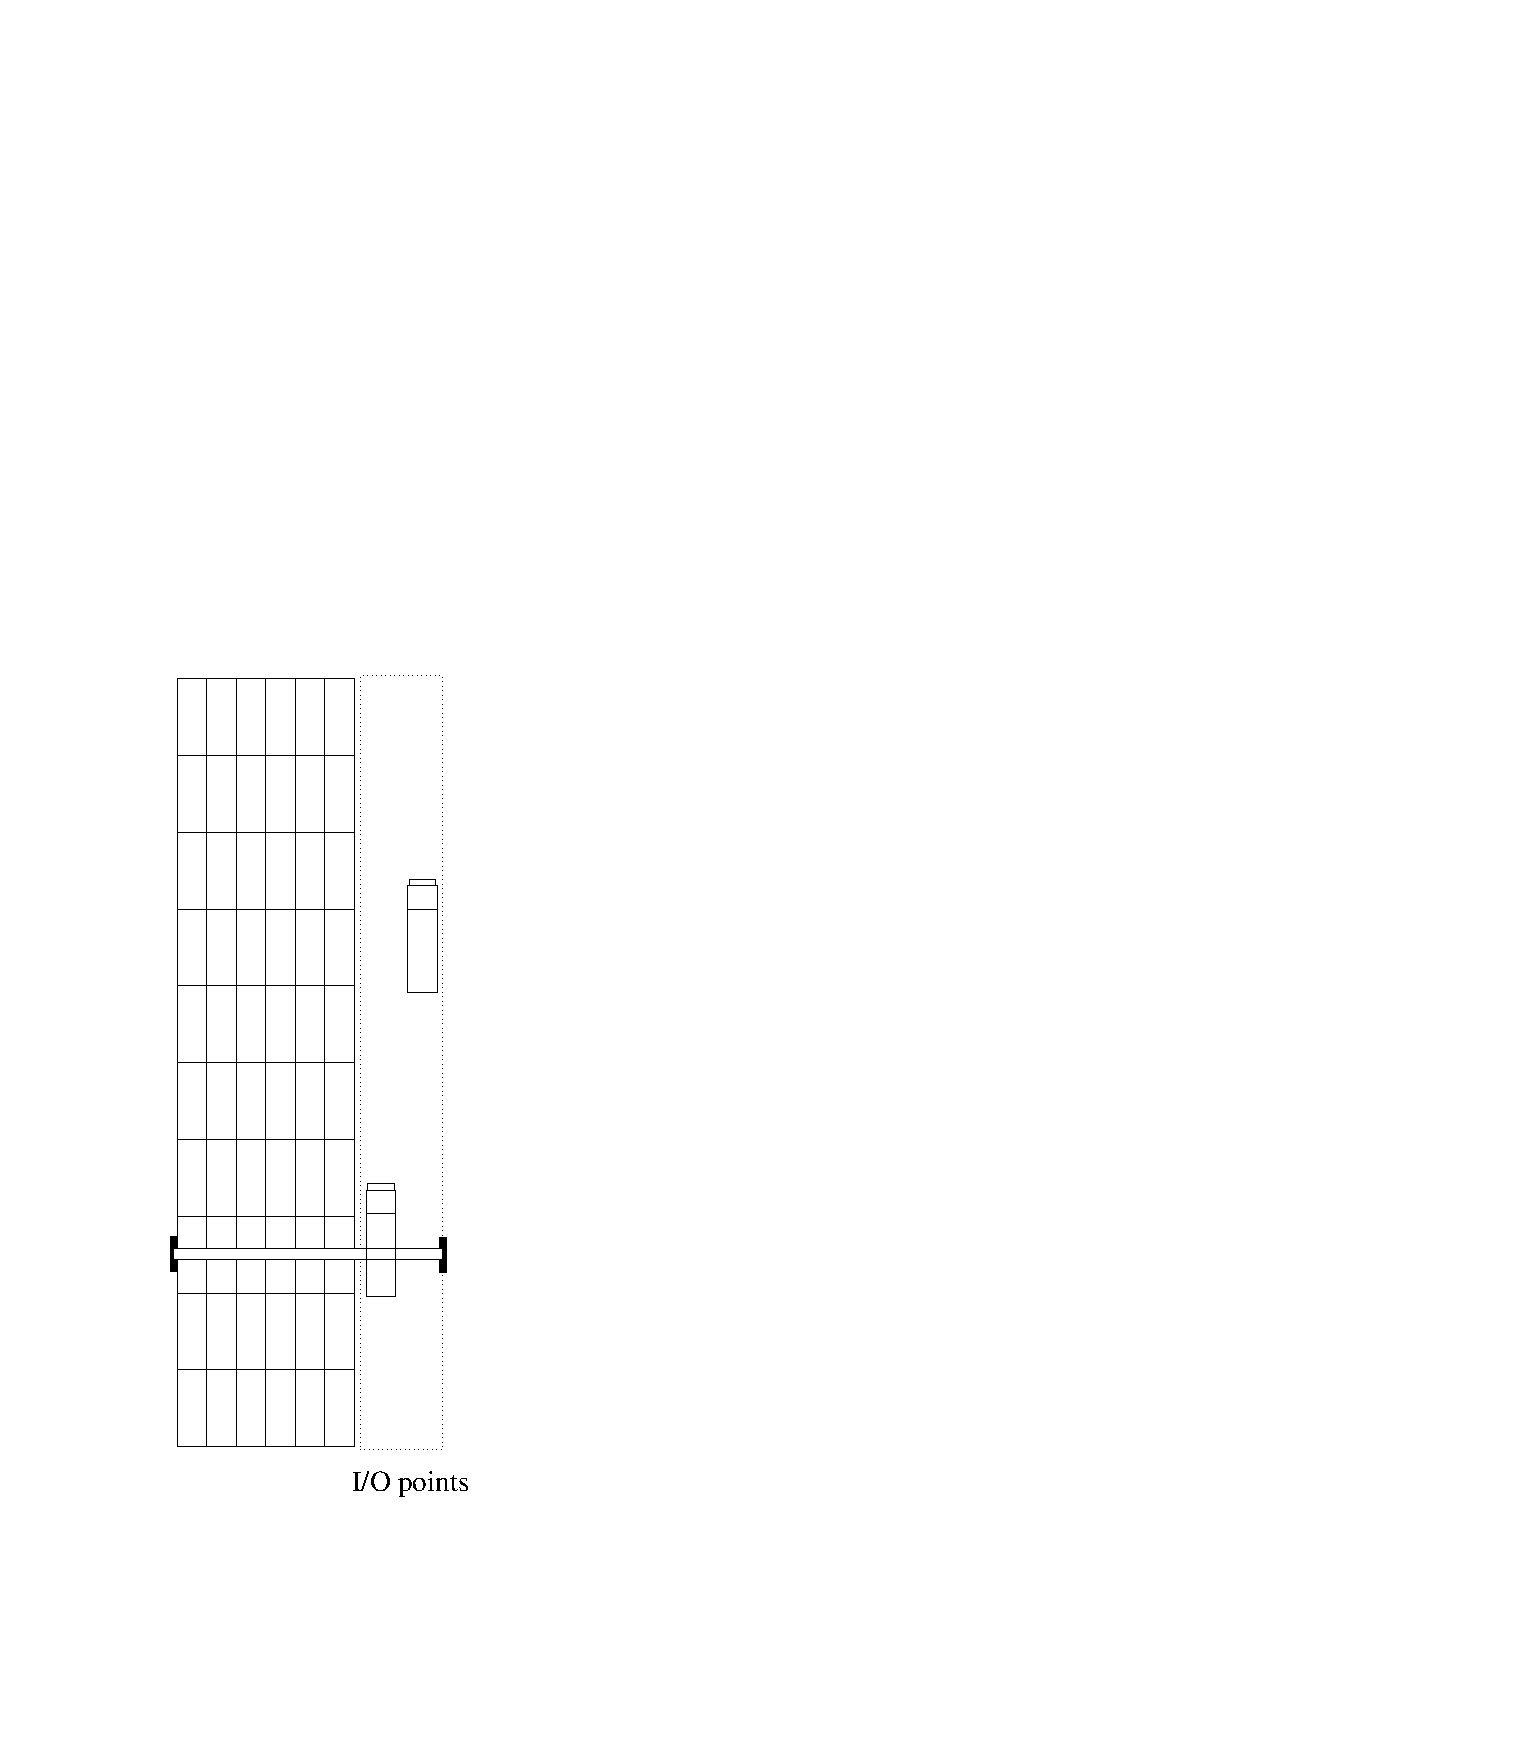
\includegraphics{fig15_1.pdf}}}
\subfigure[Layout with transfer bay]{
    \label{fig15:2}
    \resizebox{0.3 \textwidth}{!}{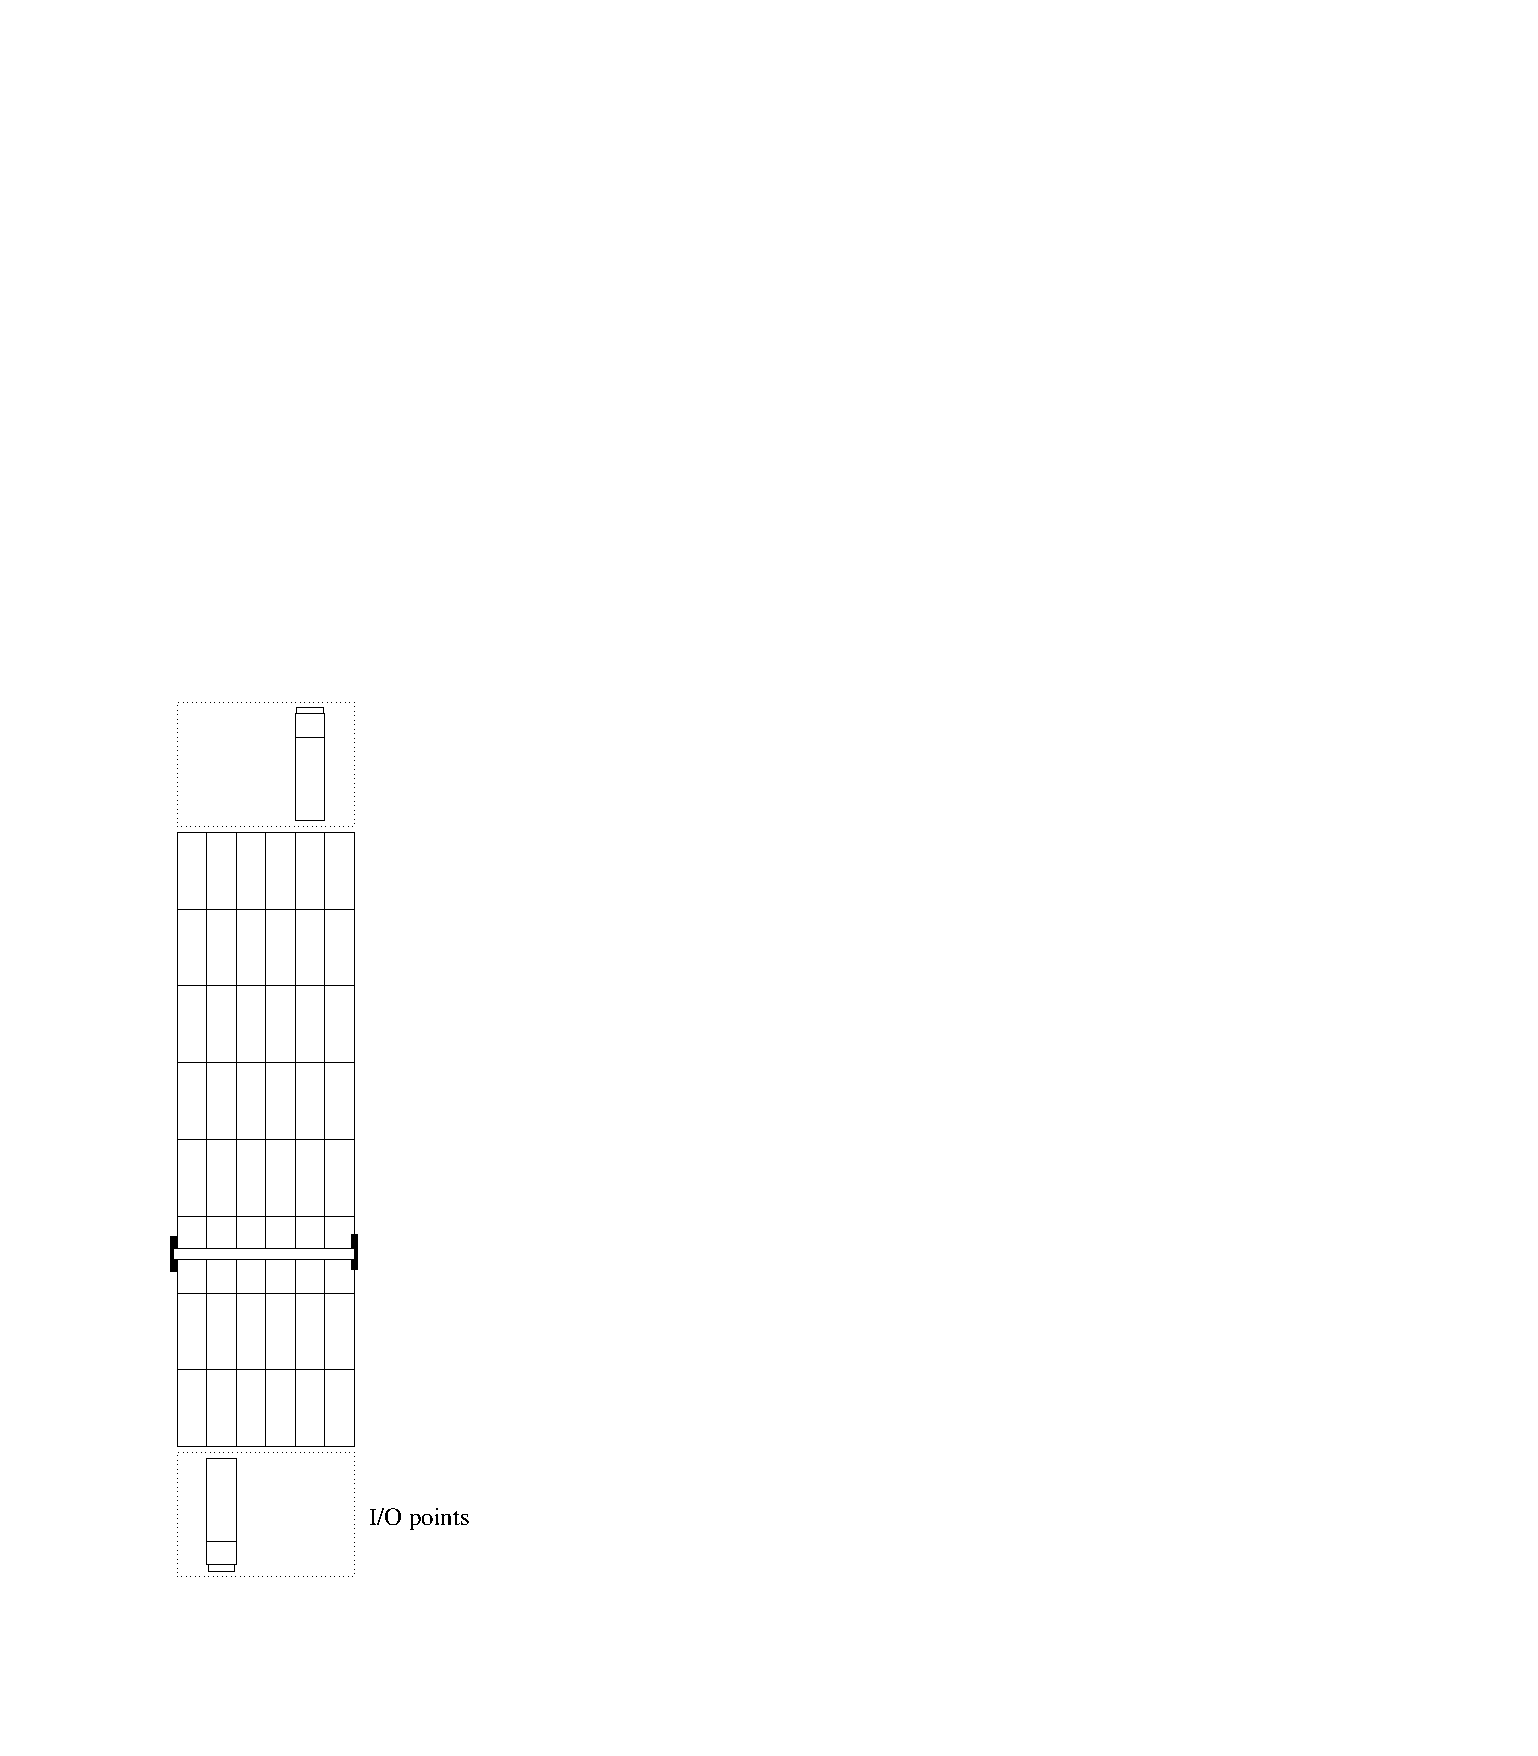
\includegraphics{fig15_2.pdf}}}
\caption{Two layouts of I/O points}
\label{fig15}
\end{figure}

Existing algorithms for CPMP have not taken dummy stacks into consideration; hence, they cannot be implemented directly at terminal layouts like Figure \ref{fig15:1}. However, aforesaid terminal layouts are popular across the world. This disparity between research and industrial practice must be resolved.

Our paper contributes to the literature in three aspects. First, CPMP is reexamined, and a new variant, that is, CPMPDS, is proposed. Second, a new lower bound suitable for both CPMP and CPMPDS is proposed. The new lower bound dominates other existing lower bounds with respect to CPMP. Third, three algorithms based on the idea of target-guided strategy are designed to solve classical CPMP and new CPMPDS. The algorithms fix containers at appropriately chosen positions and avoid moving them afterwards. This mechanism reduces the problem size continuously until the problem is solved. Thus, our algorithms guarantee termination. Experimental results demonstrate that the proposed algorithms are better than the state-of-the-art algorithm to the best of our knowledge. Although CPMP is discussed in the context of maritime terminals, it is also applicable to other scenarios, such as warehouses and railway yards.

The remainder of this paper is structured as follows. Section \ref{sec:litreview} presents an overview of existing works related to CPMP. Section \ref{sec:pd} formally defines CPMP/CPMPDS. Section \ref{sec:cf} discusses how to calculate lower bounds. A greedy algorithm and two advanced beam search algorithms are elaborated in Section \ref{sec:heu} and Section \ref{sec:g2la}, respectively. Section \ref{sec:ce} describes the experiments that were conducted to evaluate the effectiveness of the proposed algorithms and reports the results. Finally, Section \ref{sec:con} concludes the research.

\section{Literature review}
\label{sec:litreview}

In recent years, publications in press concerning terminal operations, especially container handling, have exploded. \cite{Vis2003} first provided an overview of the complex operations at container terminals and associated research problems.
\cite{Steenken2004} then provided an extensive description on main logistic processes and operations at container terminals, with a corresponding survey of optimization models and methods. \cite{Stahlbock2008} presented new updates on container terminals.
In 2014, \cite{Carlo2014} provided a new in-depth overview of storage yard operations and highlighted current industry development trends as well as associated future research directions.
Collectively, these studies point out that CPMP is an important topic and worthy of more research effort.

Most existing methods for CPMP are heuristic approaches. \cite{Caserta2009} provided a greedy heuristic based on the paradigm of corridor and roulette wheel. The corridor reduces movement choices for a certain layout and the roulette wheel provides randomness when making choices. The probability of selecting an alternative is proportional to its attractiveness.
The algorithm first builds a corridor with respect to the current layout to determine the destination stacks of a specific misplaced container. New layouts are then yielded by conducting the movements in the corridor. The attractiveness of each new layout is evaluated by an estimated number of needed relocations. A local improvement scheme is also conducted to accelerate the search process.
\cite{Exposito2012} proposed a multi-start heuristic to minimize the number of rehandles. Movements were selected by a rule called ``low priority first''. Thus, their method is more target-oriented than that of \cite{Caserta2009}. In \cite{Exposito2012}, the concepts of corridor and roulette wheel were also used in building solutions. A method was also given to generate instances and measure difficulty of instances.

Unlike the abovementioned approaches that construct solutions by finding promising movements step by step, a neighborhood search deployed by \cite{Lee2009} regards complete solutions as units of search. The neighborhood search obtains a new feasible solution by randomly modifying the current solution.
Solutions are shortened without disturbing solution feasibility by using a four-step procedure. Three minor routines were also devised to diversify the resultant solutions and reduce the number of movements. As it is very likely to generate infeasible solutions by pure modification, their method needs a large number of iterations. Hence, the method is not as efficient as the heuristic of \cite{Exposito2012}.
\cite{Huang2012heu} solved two variants of CPMP by a heuristic algorithm. One variant is commonly seen which allows containers of different groups to mix within a bay. The other variant is newly proposed, which requires containers of different groups be separately located in the final layout.

Apart from heuristics, \cite{Lee2007} developed an IP model to tackle CPMP. They converted CPMP into a multi-commodity network flow problem. A network is composed of several subnetworks. Each subnetwork represents an interim layout.
The nodes in a subnetwork correspond to slots of the bay, and containers are expressed as commodities. A solution is expressed by a flow in the network. The disadvantage of the algorithm is that the scale of networks is large even for small instances.
However, the algorithm provides an innovative view to investigate CPMP.
\cite{BF2012} thoroughly described a tree search procedure and a new lower bound for CPMP. In the search tree, solutions are constructed by compound moves (several movements) instead of single movements, and branches are classified by four movement types. The performance of the tree search is currently the best among all extant methods.
%\cite{Vob2012} gives a short note discussing an improved lower bound on the number of required container movements.

As discussed in \cite{Caserta2011}, the counterparts of CPMP include Container Re-Marshalling Problem~(CRMP) and Container Relocation Problem~(CRP). CRMP refers to reassigning containers scattered within a block into their designated bays. CRMP is not a simple extension of CPMP, because it involves multiple cranes. The interference between multiple cranes and stacking positions of containers within a bay are the difficulties of CRMP.
\cite{Caserta2011} proved that CRMP is NP-hard. \cite{Kim1998, Kang2006Plan, Park2009Plan, Choe2011} have exploited CRMP and proposed some heuristic methods to cope with it. CRP aims to retrieve containers in a predetermined order with the fewest movements. It has been studied by researchers by using various methods, ranging from meta-heuristics to simple heuristic algorithms \citep{Kim2006A, Yang2006A, Caserta2009A,Caserta2009Applying,Lee2010A,Caserta2012AM, Forster2012A, Zhu2012Iter}.


%Pre-marshalling is the preliminary work for the
%ship stowage (rf. Avriel et al. (1998) and Imai et al. (2006)); container priorities are decided by the containers
%loading order in the ship stowage.
%
%\cite{Meisel2010Con} investigate the container sequencing problem in a vessel bay. In their problem, inbound and outbound containers are exchanged between the vessel bay and yard, and they try to determine the container handling sequence so as to minimize the container handling time.
%
%\cite{Castilho1993Handling, TalebIbrahimi199313} analyze the effect of storage space and stacking strategies on the expected number of rehandles. \cite{Kim1999Segregation} deal with how to decide the height of stacks for import containers in a dynamic setting. Their objective is to minimize the number of rehandles. \cite{Kim2000} suggest a methodology to determine storage slots for every exported container in a bay while considering container weights and the layout of the bay with the objective to minimize the anticipated number of rehandles. \cite{Kang2006} propose a simulated annealing search to reduce the number of relocation movements of export containers with inaccurate weight information at the time of loading. In this work, a reduction on the number of relocations is obtained by applying a learning classifier.

\section{Problem description}
\label{sec:pd}

CPMP can be summarized as follows: Given a bay with $S$ stacks, each stack is able to store up to $H$ containers vertically. Tiers of the bay are indexed from 1 to $H$ from bottom to up. For consistency, the ground is considered as tier 0 in particular.
$N$ ($N\le S\times H$) containers are stored in the bay, which forms an initial layout with a usage rate of $N/(S\times H)$. Each container $c$ is assigned a group label $g(c)\in \{1,\dots,G\}$. The group label of different containers could be unique or duplicate. Figure \ref{fig3} shows a layout with $S=5$, $H=6$, $G=9$ and duplicate group labels.

One container can be moved from the top of a stack (\textbf{origin}) to the top of another stack (\textbf{destination}) if the destination stack is not fully occupied.
CPMP is to find the shortest movement sequence that transforms the initial layout to a final layout with all stacks \textbf{clean}. A stack is \textbf{clean} if its containers are piled in a non-increasing order of group labels from bottom to up; otherwise, the stack is \textbf{dirty}. A stack $s$ can \textbf{accommodate} a container $c$ if and only if stack $s$ is clean and is still clean when $c$ is moved to its top.
A container $c$ is a clean container if and only if all the containers underneath are clean and their group labels are no smaller than $g(c)$. Otherwise, $c$ is dirty.


\begin{figure*}[htbp]
\centering
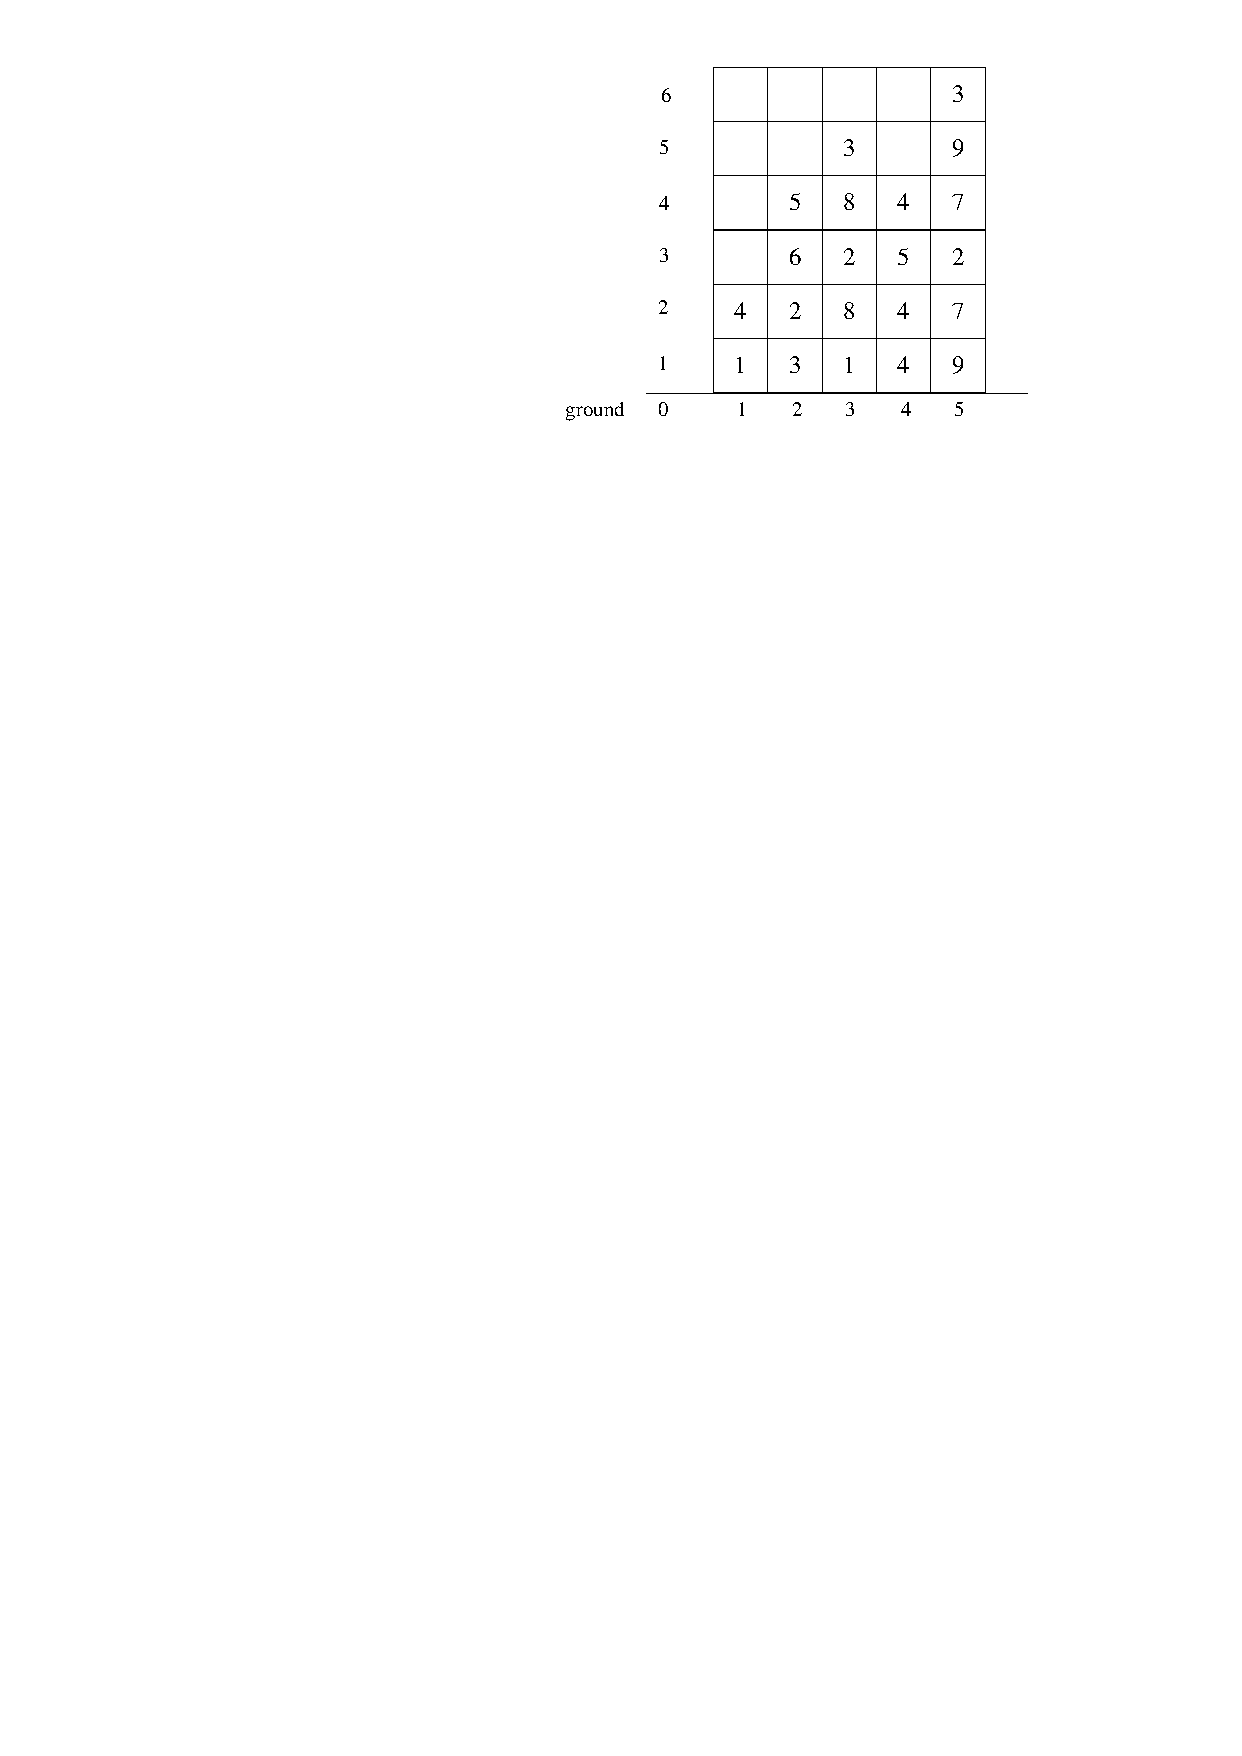
\includegraphics[width=0.4\textwidth]{fig3.pdf}
\caption{An example of a layout}
\label{fig3}
\end{figure*}

%Our paper uses the following assumptions which have been presented in \cite{Lee2007} for the resolution of the CPMP:
%\begin{enumerate}[1.]
%\item Container movements are only carried out within a single bay, i.e. movements across bays are not considered here.
%\item All the containers have the same dimensions. This is the conventional practice in container terminals.
%\item Container group labels are known in advance and do not change over time, as the ship stowage plan is determined prior to the pre-marshalling process.
%\item No container comes in or goes out of the bay when the pre-marshalling process is performed in the bay.
%\end{enumerate}

In the new variant CPMPDS, containers are only piled in the first $S-1$ stacks,and $S$-th stack (called dummy stack) is empty in the initial layout. During pre-marshalling, containers can be placed in the dummy stack. The objective of CPMPDS is to transform the initial layout to a clean layout in which the dummy stack is empty with the least movement effort. A stack is clean if it is not the dummy stack and its containers are piled in a non-increasing order of group labels from bottom to up; otherwise, it is dirty. A container $c$ is a clean container if and only if it is not placed in the dummy stack, all the containers underneath are clean, and their group labels are no smaller than $g(c)$. Otherwise, $c$ is dirty. The dummy stack cannot accommodate any containers.

For ease of illustration, some notations are defined in Table \ref{tab:1}. All the notations are used in the context of the current layout. Therefore, notations do not explicitly indicate layouts.

\begin{table}[htbp]
  \centering
  \caption{Notations}
  \label{tab:1}
    \begin{tabular}{l|l}
    \hline
    Notations         & Description \\
    \hline
    $H$               & The height limitation of a bay\\
%    $s_i$             & The $i$-th stack\\
%    $c_j$             & The $j$-th container\\
%    $l_k$             & The $k$-th layout; the initial layout is $l_0$\\
    $e(s)$            & The number of empty slots of stack $s$\\
    $h(s)$            & The number of containers of stack $s$\\
    $d(s)$            & The number of dirty containers of stack $s$\\
    $\id{uf}(s)$      & The number of unfixed containers of stack $s$\\
    $\id{sn}(c)$      & The stack where container $c$ is placed\\
    $\id{tn}(c)$      & The tier where container $c$ is placed\\
    $g(c)$            & The group label of container $c$\\
%    $\langle c,s\rangle$           & A movement which moves container $c$ to the top of $s$\\
  % $(c_1,s_1)\circ\dots\circ(c_k,s_k)$ & A movement sequence with $k$ movements\\
    $o(c)$          & The number of containers above container $c$\\
    \hline
    \end{tabular}
\end{table}



%A movement $\langle c, s\rangle$ can be applied (carried out) to a layout $l$ if and only if $s\neq \id{sn}(c,l)$, $h(s,l)<H$ and $c$ is the topmost container of a stack in $l$.
%The resultant layout is represented by $l\circ\langle c,s\rangle$. Analogically, $l \circ\langle c_1,s_1\rangle \circ \dots \circ \langle c_k,s_k\rangle$ represents the resultant layout after applying a sequence of movements $\langle c_1,s_1\rangle$, \dots, $\langle c_k,s_k\rangle$ to $l$.

%In addition, we classify the container movements into four types, just like \cite{BF2012}. A movement is a dirty-clean (DC for short) movement if a container is moved from a dirty stack to a clean stack. Similarly, the other three types are dirty-dirty  (DD), clean-dirty (CD), and clean-clean (CC). Generally, dirty-x (DX) denotes either DC or DD movements.

\section{Lower bound}
\label{sec:cf}

In this section, a new method is proposed to calculate the lower bound of the number of movements necessary to reach a clean layout. The calculation of the lower bound of CPMP is demonstrated first. The lower bound of CPMPDS requires only a small modification on the lower bound of CPMP.

%\begin{proof}
%The proof of Lemma \ref{lem:1} can be found in \cite{Wang2013Check}.
%\end{proof}
%
%\begin{theorem}
%\label{the:1}
%Given a layout with $S\ge3$, movable containers can be rearranged in any order within the whole bay.
%\end{theorem}
%\begin{proof}
%The proof of Theorem \ref{the:1} can be found in \cite{Wang2013Check}.
%\end{proof}
%
%Based on Theorem \ref{the:1}, we know that movable containers can be moved freely while immovable containers cannot be moved at all. According to Lemma \ref{lem:1}, we can separate movable containers and immovable containers at the beginning and the separation will never change, no matter what movement sequences are executed in later stages.
%Since the numbers of immovable containers in every stack are the same, if we draw a boundary line between movable and immovable containers, the line is just horizontally straight (Figure \ref{fig4}).
%%We define the slots above the boundary line as \textbf{movable slots} and the slots beneath the boundary line as \textbf{immovable slots}.
%
%\begin{figure}[htbp]
%\centering
%\subfigure[Case 1]{
%    \label{fig4:1}
%    \resizebox{0.3 \textwidth}{!}{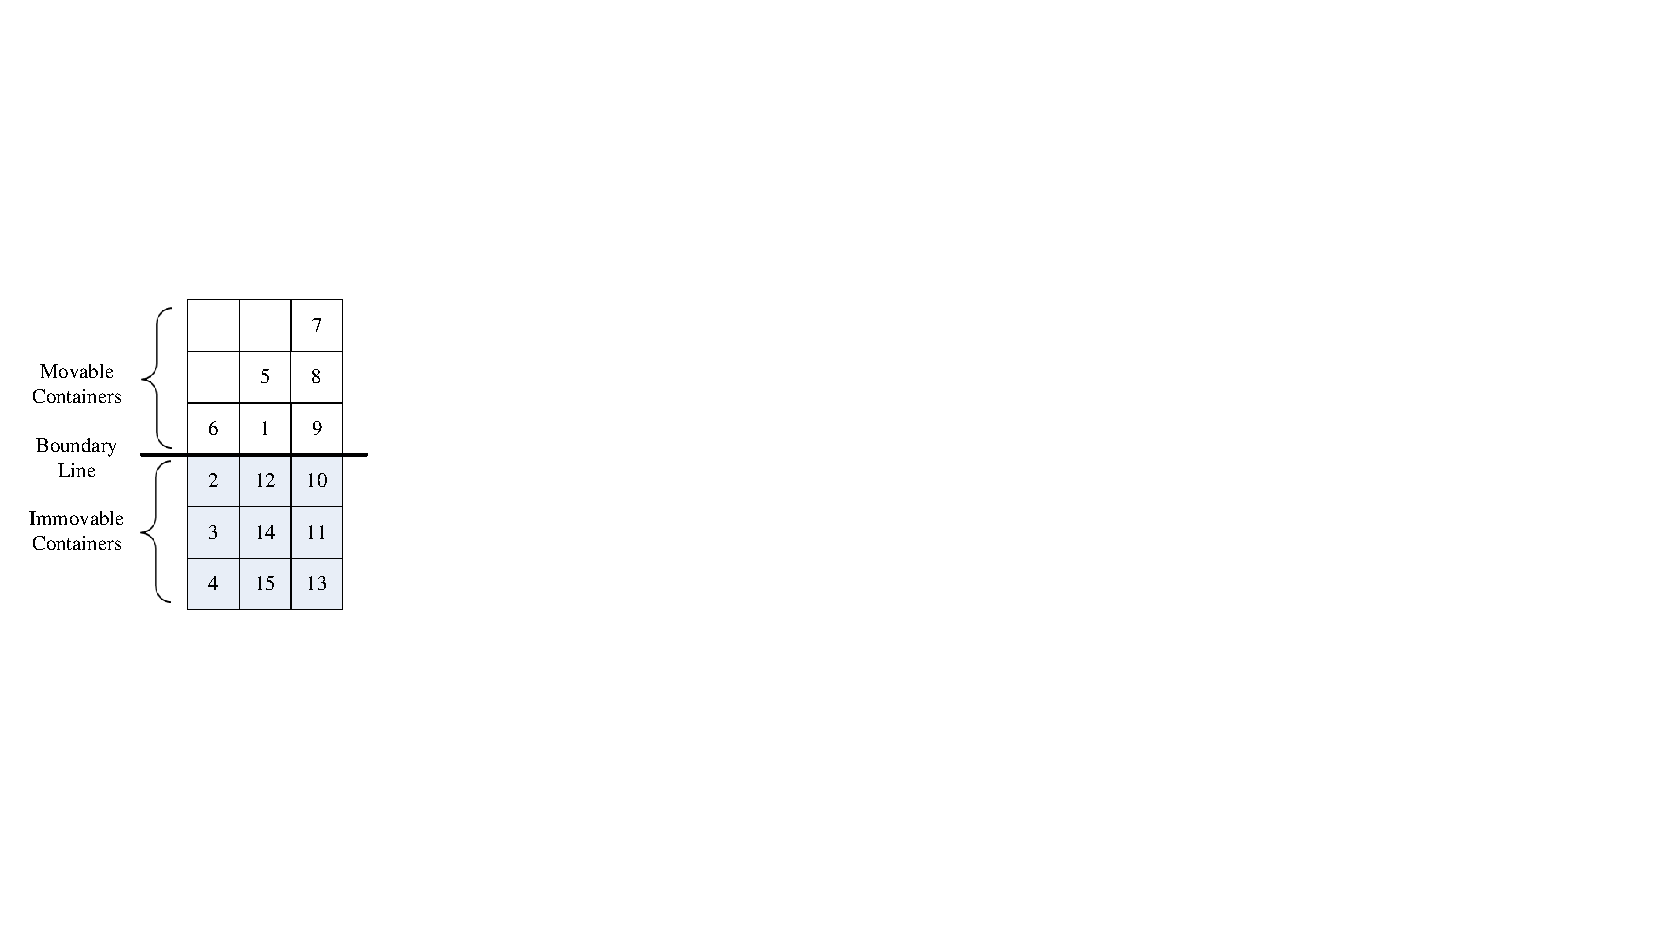
\includegraphics{fig4_1.pdf}}}
%\subfigure[Case 2]{
%    \label{fig10:2}
%    \resizebox{0.3 \textwidth}{!}{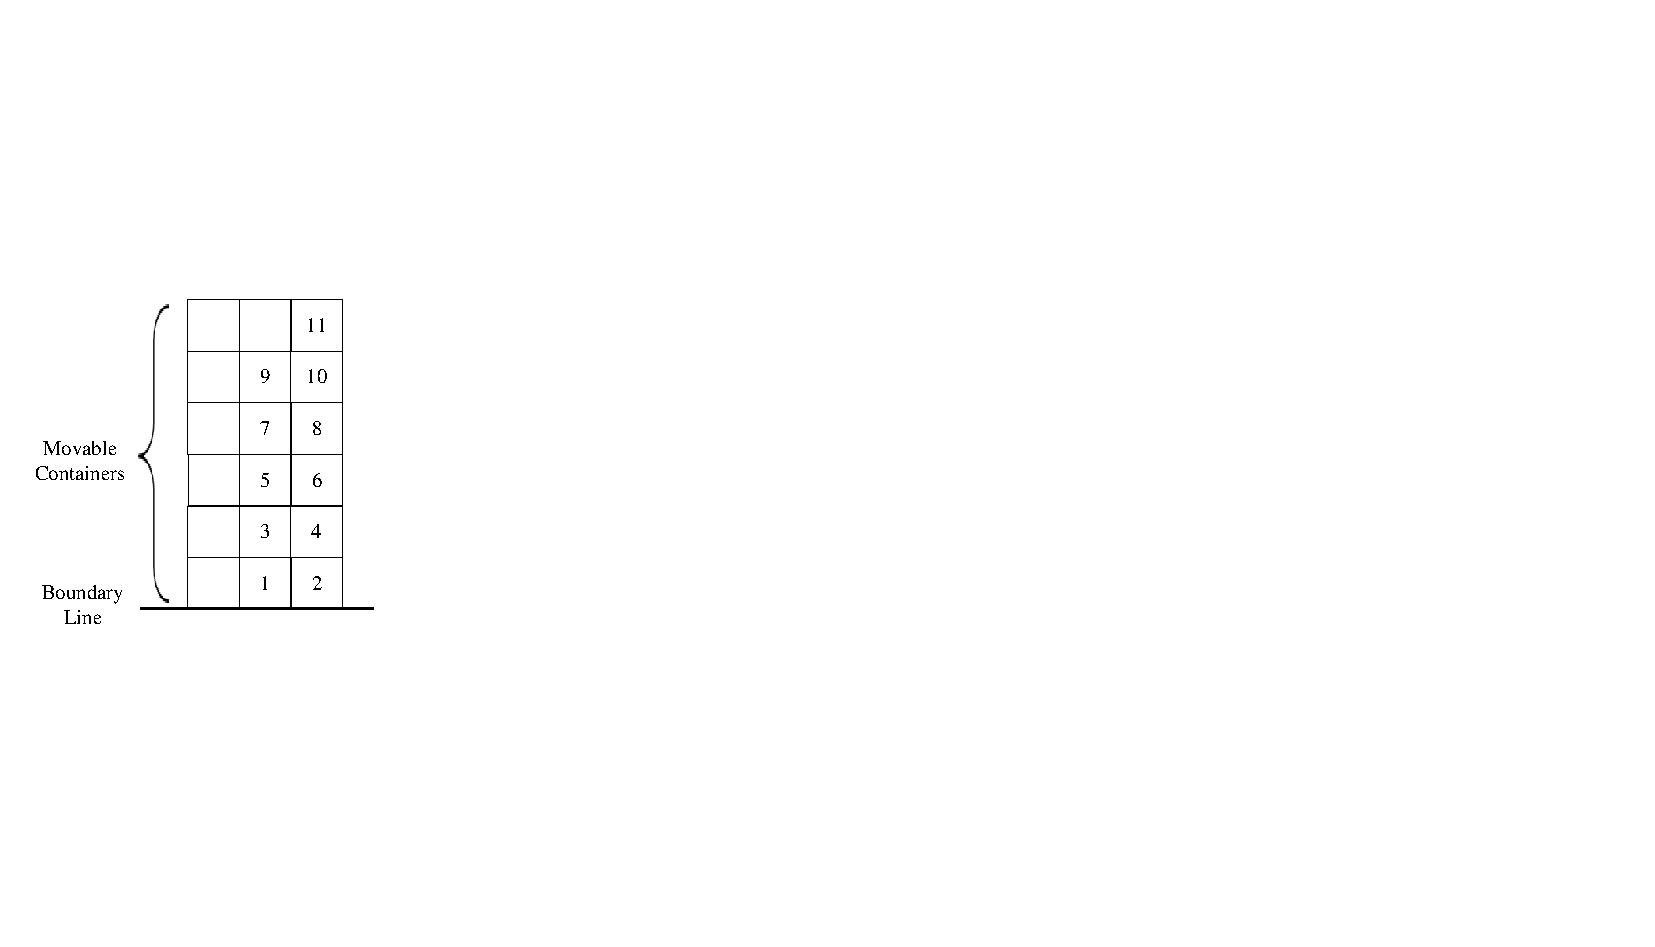
\includegraphics{fig4_2.pdf}}}
%\caption{Boundary Line}
%\label{fig4}
%\end{figure}


%\subsection{Feasibility check}
%
%The feasibility of any CPMP/CPMPDS instance depends on the existence of a solution (movement sequence) that can transform the initial layout to a feasible layout.
%
%\subsubsection{CPMP instances}
%
%For any CPMP instance with $S=2$, a dirty layout is feasible if and only if: one stack $s_1$ is dirty, and the other stack $s_2$ is clean.
%Stack $s_1$ has two parts: the lower part and the higher part, where containers have a non-increasing order and non-decreasing order of group labels from bottom to up, respectively.
%In addition, the size of the higher part must be no larger than $e(s_2)$, and stack $s_2$ can accommodate the topmost container of stack $s_1$.
%
%For any CPMP instance with $S\ge3$, all movable containers can be rearranged in any order based on Theorem \ref{the:1}.
%The instance is concluded to be feasible if all stacks have no immovable containers.
%Otherwise, all movable containers are removed to determine if they can be piled on the left immovable containers, which results in a clean layout regardless of the specific movement sequence. $G$-dimensional vectors $\mathbf S$ and $\mathbf D$ are introduced to this end to record slot supply and demand above the boundary line, respectively.
%Initially, all elements of $\mathbf S$ and $\mathbf D$ are zero. For each stack $s$, $H-\id{im}$ is added to element $\mathbf S_g$ if the group label of its topmost immovable container is $g$.
%The notation $\id{im}$ from Lemma \ref{lem:1} is the number of immovable containers in a stack. Element $\mathbf D_g$ of $\mathbf D$ records the number of movable containers with group label $g$.
%
%An instance is feasible if and only if the demand of each group does not exceed the supply of the corresponding group, namely, $\mathbf S_g+\sum\limits_{i>g}\mathbf S_i-\sum\limits_{i>g}\mathbf D_i\ge \mathbf D_g$.
%In another word, an instance is feasible if and only if the surplus for each group is non-negative, i.e.,
%\begin{equation}
%\label{equ:2}
%\sum\limits_{i\ge g}\mathbf S_i-\sum\limits_{i\ge g}\mathbf D_i\ge0, \quad g=1,\dots,G
%\end{equation}
%
%\subsubsection{CPMPDS instances}
%
%Any CPMPDS instance with $S=2$ is feasible if and only if the initial layout is feasible. Let stack $s_2$ be the dummy stack and stack $s_1$ be the other stack. A noteworthy case is that containers are piled in a non-decreasing order of group labels from bottom to up in stack $s_1$, and stack $s_2$ is empty. Although all containers can be relocated to stack $s_2$ one by one, which results in a clean layout with stack $s_1$ empty, the case is still infeasible in our opinion because stack $s_2$ should be empty in the final layout. This condition cannot be changed in any way, because the position of trucks cannot change.
%
%All CPMPDS instances with $S\ge3$ are feasible. The number of immovable containers $\id{im}=0$, because an empty dummy stack exists. All containers can be rearranged in any order.
%%Then they must can be rearranged in an order where all containers within a stack are piled in a decreasing order of group labels from the bottom up which is a feasible final layout.
%Thus, any CPMPDS instance with $S\ge3$ is feasible.


\subsection{Lower bound of CPMP}

The lower bound is obtained by estimating the number of movements that belong to different movement types.
\begin{enumerate}
\setcounter{enumi}{0}
\item Dirty--Clean movements
\end{enumerate}

The number of dirty containers in a given layout is $\sum\limits_{s=1}^S d(s)$. Each dirty container requires at least one movement to become clean; thus, the lower bound of the number of Dirty--Clean movements is $\id{num}_\id{DC}=\sum\limits_{s=1}^S d(s)$.

\begin{enumerate}
\setcounter{enumi}{1}
\item Dirty--Dirty movements
\end{enumerate}

If all stacks are dirty in a layout, at least one stack should become clean to accommodate containers. This step is done by moving dirty containers of a stack to other dirty stacks. The least number of such Dirty--Dirty movements is $\id{num}_\id{DD} = \min\limits_s d(s)$.

\begin{enumerate}
\setcounter{enumi}{2}
\item Clean--X movements
\end{enumerate}

Before proceeding to explain the calculation, the concept of skyline is first introduced. A skyline is any vertical partition that separates a layout into higher and lower parts, where the lower part must be clean. A skyline can be represented by a vector $\id{SL}$ such that each element $\id{SL}_s$ represents the skyline segment across stack $s$. Segment $\id{SL}_s$ is described by the container underneath; the tier and group numbers of $\id{SL}_s$ are equal to those of the associated container. For example, in Figure \ref{fig5}, the bold line presents a skyline of the layout with $\id{tn}(\id{SL}_{2})=3$ and $g(\id{SL}_{2})=1$.


\begin{figure*}[htbp]
\centering
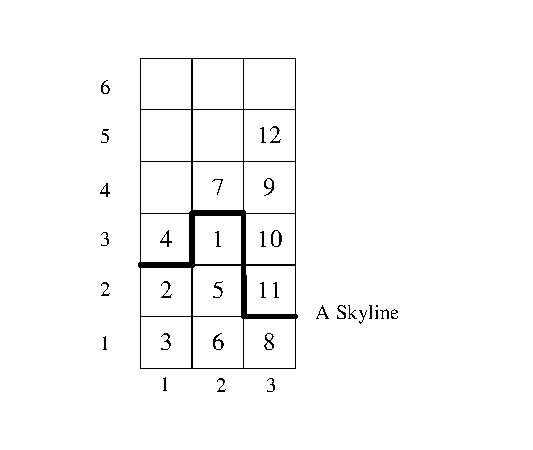
\includegraphics[width=0.3\textwidth]{fig5.pdf}
\caption{A skyline of a layout}
\label{fig5}
\end{figure*}

Supply and demand vectors, denoted as $\mathbf S^\id{SL}$ and $\mathbf D^\id{SL}$, record the numbers of slots and containers above \id{SL}. The $g$-th element of $\mathbf S^\id{SL}$ is $\mathbf S^\id{SL}_g=\sum\limits_{s:g(\id{SL}_s)=g}H-\id{tn}(\id{SL}_s)$, whereas the $g$-th element of $\mathbf D^\id{SL}$ is the number of containers above $\id{SL}$ with group labels $g$.

For ease of explanation, Clean--Dirty and Clean--Clean movements are merged as Clean--X movements. The number of moved clean containers is a lower bound of the number of Clean--X movements. Ideally, pre-marshalling work involves dirty containers only and leaves clean containers unmoved. In some cases, however, achieving a clean layout is impossible without moving clean containers. The number of clean containers that need to be moved can be counted by the following process: given a bay, all dirty containers and a set of clean containers $C$ are removed from the layout, then slots are reassigned to removed containers. The resultant layout is required to be clean. Removed containers within a stack should be consecutive, i.e., if two containers from the same stack are removed, containers between them are also removed. The size of smallest $C$ is the number of Clean--X movements $\id{num}_{CX}$. Finding the smallest $C$ is equivalent to finding the skyline with the fewest clean containers in its higher part (smallest skyline) as well as non-negative surpluses (Equation \ref{equ:3}).

\begin{equation}
\label{equ:3}
\sum\limits_{i\ge g}\mathbf S^\id{SL}_i-\sum\limits_{i\ge g}\mathbf D^\id{SL}_i\ge0, \quad g=1,\dots,G
\end{equation}

To find the smallest skyline, a basic skyline $\id{SL}$ that separates clean and dirty containers is drawn. Next, a depth-first-search (DFS) is deployed to push a certain segment of $\id{SL}$ one tier down in each branching. The leaves of the search tree are all the skylines with non-negative surpluses; the one with the fewest pushes is selected and the number of pushes is $\id{num}_\id{CX}$.

To conclude, the lower bound can be defined as $\id{LB}_\id{DFS}=\id{num}_\id{DC}+\id{num}_\id{DD}+\id{num}_\id{CX}$.

\subsection{Clean--X movements by maximum knapsack}

The lower bound $\id{LB}_\id{DFS}$ is time consuming because a DFS is used to calculate $\id{num}_{\id{CX}}$. A maximum knapsack method (MKM) is proposed to approximate $\id{num}_{CX}$. A basic skyline SL that separates clean and dirty containers is drawn, then the smallest skyline with non-negative surplus for a single group is obtained instead of for all groups. This search is repeated for each group, and the largest number of pushes is selected amongst all obtained skylines.

For a given group label $g$, a knapsack-like problem is solved to find the smallest skyline with non-negative surplus in terms of $g$. Stacks in the bay are regarded as items, where each item $s\in\{1,\dots,S\}$ has value $v_s$ and cost $c_s$. The objective is to select a set of items with the lowest cost such that the total value selected is at least $V$. Every item can only be selected at most once. $c_s$ is the number of clean containers in stack $s$ to be moved to accommodate group $g$, while $v_s$ is the resultant number of slots available for group $g$, i.e., $v_s=c_s+e(s)$. $V$ is the number of dirty containers with group labels $g(c)\ge g$. The decision variable $x_s$ is 1 if stack $s$ is selected; otherwise, $x_s=0$. The integer programming model of this knapsack-like problem is show in Equation \ref{equ:4} and can be solved easily by dynamic programming.


\begin{equation}
\label{equ:4}
\begin{array}{rl}
\min & \sum\limits_{s=1}^S c_s x_s\\
\mathrm{s.t.} &\sum\limits_{s=1}^S v_s x_s\ge V\\
&x_s\in\{0,1\}, \quad s=1,\dots,S
\end{array}
\end{equation}

MKM is not as precise as DFS, but the solution gap is quite small and the computation speed is improved. The lower bound provided by MKM is denoted as $\id{LB}_{\id{MKM}}$.

\subsection{Comparison with existing lower bound}
The current state-of-the-art lower bound $\id{LB}_\id{BF}$ was proposed by \cite{BF2012}, which also consists of three parts: Dirty--Clean, Dirty--Dirty and Clean--X movements.
The first two types are calculated in the same manner as $\id{LB}_\id{DFS}$ and $\id{LB}_\id{MKM}$ in this paper. For Clean--X movements, a basic skyline SL that separates clean and dirty containers is drawn, then they only take the group label $g^*$ with the smallest surplus $\id{min}=\min\limits_g\sum\limits_{i\ge g}\mathbf S^\id{SL}_i-\sum\limits_{i\ge g}\mathbf D^\id{SL}_i$. If $\id{min}$ is negative, $\sum\limits_{i\ge g^*}\mathbf D^\id{SL}_i$ surpasses $\sum\limits_{i\ge g^*}\mathbf S^\id{SL}_i$ by $|\id{min}|$, which means that clean containers need to be moved to accommodate these $|\id{min}|$ dirty containers. The number of moved clean containers $\id{num}_\id{CX}$ is estimated by \cite{BF2012} as follows: suppose one stack is able to (although in fact it may not be able to) accommodate $H$ dirty containers with $g\ge g^*$, then $|\id{min}|$ dirty containers need at least $\left\lceil\frac{|\id{min}|}{H}\right\rceil$ stacks. As slots supply of stacks with $g(\id{SL}_s)\ge g^*$ have been calculated into $\sum\limits_{i\ge g^*}\mathbf S^\id{SL}_i$, only stacks with $g(\id{SL}_s)< g^*$ (denote as set \id{AS}) can provide slots for $|\id{min}|$ dirty containers. Suppose $c_s$ is the number of clean containers in stack $s$ to be moved to accommodate group $g^*$, sort stacks in set $\id{AS}$ by ascending values of $c_s$. The first $\left\lceil\frac{|\id{min}|}{H}\right\rceil$ stacks are selected and $\id{num}_\id{CX}=\sum\limits_{s=1}^{s=\left\lceil\frac{|\id{min}|}{H}\right\rceil}c_s$.

From the mathematical perspective, the method of \cite{BF2012} is equivalent to solving the following model: stacks in the bay are regarded as items, where each item $s\in\{1,\dots,S\}$ has value $v_s'$ and cost $c_s$. The objective is to select a set of items with the lowest cost such that the total value selected is at least $V$. Every item can only be selected at most once. $c_s$ is the number of clean containers in stack $s$ to be moved to accommodate group $g^*$, while $v_s'$ is the resultant number of slots available for group $g^*$. According to \cite{BF2012}, $v_s'=H$ if $g(\id{SL}_s)<g^*$; otherwise, $v_s'=c_s+e(s)$. $V$ is the number of dirty containers with group labels $g(c)\ge g^*$. The decision variable $x_s$ is 1 if stack $s$ is selected; otherwise, $x_s=0$. The integer programming model is show in Equation \ref{equ:5}.


\begin{equation}
\label{equ:5}
\begin{array}{rl}
\min & \sum\limits_{s=1}^S c_s x_s\\
\mathrm{s.t.} &\sum\limits_{s=1}^S v_s' x_s\ge V\\
&x_s\in\{0,1\}, \quad s=1,\dots,S
\end{array}
\end{equation}

Compare Model \ref{equ:4} with Model \ref{equ:5}, all parameters are the same except $v_s$ ($v_s'$). As $v_s\le v_s'$ for and $s$, the solution to Model \ref{equ:5} is the solution to Model \ref{equ:4}, while the reverse does not stand. The solution space of Model \ref{equ:5} is larger than Model \ref{equ:4}, thus the optimal solution to Model \ref{equ:4} is no smaller than that to Model \ref{equ:5}. Furthermore, \cite{BF2012} only solve Model \ref{equ:5} once for $g^*$, whereas this paper solves Model \ref{equ:4} for every group and then takes the maximal result as $\id{num}_\id{CX}$. As a result, the lower bound $\id{LB}_\id{MKM}$ dominates $\id{LB}_\id{BF}$: $\id{LB}_\id{BF}\le \id{LB}_\id{MKM}\le \id{LB}_\id{DFS}$.
\subsection{Lower bound of CPMPDS}

The lower bound of CPMPDS consists of three parts: Dirty--Clean, Dirty--Dirty, and Clean--X movements.

The lower bound of Dirty--Clean movements is equal to the number of dirty containers. For Dirty--Dirty movements, $\id{num}_\id{DD}=\min\limits_{s\neq s_d} d(s)$, where $s_d$ is the dummy stack. If all stacks except the dummy stack are dirty, then dirty containers from at least one stack need to be relocated to other dirty stacks or the dummy stack. In both situations, these containers are still dirty after relocation.

The lower bound of Clean--X movements is the number of clean containers moved to make all containers clean and dummy stack empty, which is equivalent to assigning containers only to the first $S-1$ stacks and ignoring the dummy stack.

Based on the analysis above, $\id{LB}_\id{DFS}$ ($\id{LB}_\id{MKM}$) of a CPMPDS instance is equal to $\id{LB}_\id{DFS}$ ($\id{LB}_\id{MKM}$) of the corresponding CPMP instance with the dummy stack removed.

\section{Target-guided heuristic}
\label{sec:heu}

This section presents a target-guided heuristic (TGH) for CPMP/CPMPDS. This heuristic can be used as an independent algorithm as well as a component of more complex algorithms in the next section. Before proceeding to the heuristic, the concept of movable (immovable) containers is introduced.

\begin{definition}
\label{def:1}
A container is movable if it can be fetched and replaced to another stack.
\end{definition}

In a given layout, for any stack $s$, only the top $\sum\limits_{i\neq s}e(i)$ containers are movable. Other containers in $s$, if any, are immovable; the numbers of immovable containers in every stack are the same, which are equal to $\id{im}=\max\left\{0, H-\sum\limits_{s=1}^S e(s)\right\}$.

The main idea of the heuristic is to fix one container in a certain slot at a time starting from the largest group label. After a container is fixed, only a special case will be able to relocate it. The special case is solved by relocating fixed containers back; this action will be explained later.
As containers are fixed continuously, all stacks become clean in the end. Hence, this heuristic guarantees a solution for any feasible instance. A complete description of the framework is shown in Algorithm \ref{alg:heu}.
%It suits both the CPMP and the CPMPDS.

\begin{algorithm}[htbp]
	\caption{The target-guided heuristic for CPMP/CPMPDS}
	\label{alg:heu}
	\begin{codebox}
	\Procname{\proc{TGH (\id{inilay})}}
	\li $\id{curlay} = \id{inilay}$
    \li $\id{conList}$ = NULL
    \li $\id{stkList}$ = NULL
    \li mark all the immovable containers in \id{curlay} as fixed
    \li mark all the movable containers in \id{curlay} as unfixed
    \li $\id{g} = G$
    \li \While $g\neq0$
    \li \Do
            mark clean containers with group labels \id{g} as fixed\label{heu:c}
    \li     \id{conList} = the set of candidate containers
    \li     \While $\id{conList} \neq \emptyset$\label{heu:l}
    \li     \Do
                \id{stkList} = the set of candidate stacks
    \li         select the target container and stack from \id{conList} and \id{stkList}, respectively
    \li         apply a giant move to fix the target container to the target stack
            \End
    \li $g=g-1$
        \End
%	\li \Return;
	\end{codebox}	
\end{algorithm}

%The heuristic starts with the initial layout $\id{inilay}$. In the initialization stage, all the immovable containers are labeled as fixed while movable containers as unfixed.
%The current layout $\id{curlay}$ is initialized with $\id{inilay}$ and current group $g$ is initialized with $G$. In the following, the algorithm fixes containers one by one according to a descending order of group numbers.
%When fixing containers with a certain group label, clean containers are fixed in their original positions directly and marked as fixed (Line \ref{heu:c}).
%For the dirty containers, we fix them successively. In the current layout, we select one target container and one target stack, and apply several movements so as to fix the target container to the target stack, resulting a new layout. Such a process is called one transition.
In Algorithm \ref{alg:heu}, a movement sequence that fixes a target container to a target stack is named as a \textbf{giant move}. By contract, a one-movement operation is coined as a \textbf{baby move}.

The advantage of the proposed heuristic is that containers are fixed one by one. Therefore, customizing the heuristic for other CPMP variants, i.e., variants that require containers in a final layout adhere to special distribution characteristics, is easy. The heuristic only needs to modify the rules of candidate stack selection to fix containers according to the required distribution.



\subsection{Candidate container and stack selection}
\label{sec:can}
The set of candidate containers when processing group $g$ comprises all unfixed containers with group labels $g$. A set of candidate stacks are selected based on the set of candidate containers and each candidate stack must be able to accommodate group $g$ after relocating some of its containers.
%For example, in Figure \ref{fig4:1}, the available stack for container 6 is only the stack in the middle.
Among all available stacks, stacks that can accommodate $g$ without any relocation is preferred; otherwise, other stacks are selected.

\subsection{Target pair selection}
\label{sec:tar}
An evaluation scheme is designed to evaluate the attractiveness of fixing a candidate container to a candidate stack.
%The candidate containers are from \id{conList}, and the candidate stacks are the result from procedure \proc{CandidateStack}.
%The attractiveness of each candidate pair $(c,s)$ is evaluated by an evaluation scheme and the most attractive pair is selected as the target container \id{con} and target stack \id{stk}, respectively.
Intuitively, fewer movements for fixing is preferred. A function $f(c,s)$ is introduced to roughly estimate the movement cost for fixing container $c$ to stack $s$. If $c$ is currently in $s$, $f(c,s)=\id{uf}(s)$; otherwise, $f(c,s)=\id{uf}(s)+o(c)$. Stacks with smaller numbers of fixed containers $h(s)-\id{uf}(s)$ are preferred. This preference distributes fixed containers evenly among stacks. Thus, 2-tuple $(f(c,s), h(s)-\id{uf}(s))$ evaluates the attractiveness.

Each candidate container and each candidate stack make up a candidate pair. All the candidate pairs are sorted in an ascending lexicographical order of evaluation values, and the best one is selected as the target pair.

\subsection{A giant move}

Given target container $c^*$ and target stack $s^*$, a giant move is executed to fix $c^*$ in $s^*$. The target slot in $s^*$ for $c^*$ is the slot just above fixed containers of $s^*$. Hereafter, the target slot will not be explicitly pointed out, because a giant move does not disturb positions of fixed containers. According to whether the origin of $c^*$ is $s^*$ or not, the giant move includes two cases. 

\subsubsection{Case 1: Fixing to the same stack}

In Case 1, the origin of $c^*$ is $s^*$. In the first step, all containers above $c^*$ are relocated; the relocation strategy will be explained in Section \ref{sec:rel}. After that, $c^*$ is at the top of $s^*$ and needs a stack for temporary storage. The highest non-full stacks are considered for temporary storage. Among such stacks, a dirty stack is preferred, denoted as $\id{ts}$.

Before moving $c^*$ to $\id{ts}$, observe in advance the relocation positions of unfixed containers under $c^*$ so that $s^*$ can accommodate $c^*$. Avoiding occupying both $\id{ts}$ and $s^*$ is a straightforward idea. On top of this, denote the set of stacks except $\id{ts}$ and $s^*$ as $\id{AS}$, compute its available empty slots $\id{nslot} = \sum\limits_{s\in \id{AS}}e(s)$, and compare $\id{nslot}$ with $\id{uf}(s^*)$. According to comparison results, three scenarios are raised.

\begin{enumerate}
\setcounter{enumi}{0}
\item $\id{nslot}\ge \id{uf}(s^*)-1$
\end{enumerate}
In this scenario, the empty slots of $\id{AS}$ are enough to store unfixed containers under $c^*$. $c^*$ is moved directly to $\id{ts}$, then all unfixed containers of $s^*$ are relocated to empty slots of $\id{AS}$. Finally, $c^*$ is moved back to $s^*$.

\begin{enumerate}
\setcounter{enumi}{1}
\item $0<\id{nslot}< \id{uf}(s^*)-1$
\end{enumerate}
In this scenario, the empty slots of $\id{AS}$ are not enough for unfixed containers under $c^*$. After moving $c^*$ to $\id{ts}$, only the first $\id{nslot}-1$ unfixed containers are relocated to the empty slots of $\id{AS}$, leaving one empty slot. The last empty slot is occupied by moving $c^*$ to it. The remaining unfixed containers in $s^*$ are then relocated to $\id{ts}$. At last, $c^*$ is moved back to $s^*$.
\begin{enumerate}
\setcounter{enumi}{2}
\item $\id{nslot}=0$
\end{enumerate}
In this scenario, all stacks in \id{AS} are full. $c^*$ cannot be moved directly to \id{ts}; otherwise, it will be buried by unfixed containers in $s^*$. A top slot is needed to temporarily store $c^*$. To create such an empty slot, a top container $c$ is found from all top containers of stacks in \id{AS}.

If \id{ts} is a clean stack, the preference is as follows:
\begin{enumerate}[1.]
\item Among dirty containers that \id{ts} can accommodate, the one with the largest group label is selected;
\item Among clean containers that \id{ts} can accommodate, the one with the largest group label is selected;
\item The dirty container with the smallest group label is selected;
\item The clean container with the smallest group label is selected.
\end{enumerate}

If \id{ts} is a dirty stack, the preference is:
\begin{enumerate}[1.]
\item The dirty container with the smallest group label is selected;
\item The clean container with the smallest group label is selected.
\end{enumerate}
After $c$ is moved to $\id{ts}$, its origin is occupied by $c^*$. All unfixed containers of $s^*$ are relocated to $\id{ts}$. Finally, $c^*$ is moved to $s^*$. If $c$ is a fixed container, it is restored to its origin. Suppose the origin of $c$ is stack \id{cs}, all containers above $c$ are relocated and $c$ is moved back to \id{cs}.
%\begin{algorithm}[htbp]
%	\caption{Fix the target container to the same stack}
%	\label{alg:fixs}
%	\begin{codebox}
%	\Procname{\proc{FixS(\id{con}, \id{curlay})}}
%    \li $\id{os}=\id{sn}(\id{con})$ and \id{g} = $g(\id{con})$;
%    \li \id{curlay} = \proc{Move\_Containers($O(\id{con})$, \id{g}, $-1$)};
%    \li \id{ts} = select a non-full stack with the highest height, and prefer a dirty stack among such stacks;
%    \li \id{nslot} = $\sum_{s\neq \id{os},\id{ts}}e(s,\id{curlay})$;
%    \li \If ($\id{nslot}\ge \id{uf}(\id{os}, \id{curlay})-1$)
%    \li     \Then
%            Put \id{con} to the top of stack \id{ts} and update \id{curlay};
%    \li     \id{curlay} = \proc{Move\_Containers($\id{uf}(\id{os},\id{curlay})$, \id{g}, \id{ts})};
%    \li     Put \id{con} to the top of stack \id{os} and update \id{curlay};
%    \li \ElseIf ($\id{nslot}>0$)
%    \li     \Then
%            Put \id{con} to the top of stack \id{ts} and update \id{curlay};
%    \li     \id{C} = set of the top $nslot-1$ containers of stack \id{os};
%    \li     \id{curlay} = \proc{Move\_Containers(\id{C}, \id{g}, \id{ts})};
%    \li     Put \id{con} to $S\backslash \{\id{os}, \id{ts}$\} and update \id{curlay};{\color{red}what does this line mean?}
%    \li     \id{curlay} = \proc{Move\_Containers($\id{uf}(\id{os}, \id{curlay})$, \id{g}, $-1$)};
%    \li     Put \id{con} to the top of stack \id{os} and update \id{curlay};
%    \li \Else
%    \li     \id{ts2} = select a full stack with parameter \id{ts} according to rule R;\label{fixs:r}
%    \li     \id{c^*} = the top container of stack \id{ts2};
%    \li     Put \id{c^*} to stack \id{ts}, put \id{con} to stack \id{ts2}, and update \id{curlay};
%    \li     \id{curlay} = \proc{Move\_Containers($\id{uf}(\id{os}, \id{curlay})$, \id{g}, $-1$)};
%    \li     Put \id{con} to the top of stack \id{os} and update \id{curlay};
%    \li     \If(\id{c^*} was fixed)\label{fixs:ms}
%    \li         \Then
%                \id{curlay} = \proc{Move\_Containers($O(c^*)$, \id{g}, \id{ts2})};
%    \li         Put \id{c^*} to stack \id{ts2} and update \id{curlay};\label{fixs:me}
%            \End
%        \End
%    \li \Return \id{curlay};
%	\end{codebox}	
%\end{algorithm}
\subsubsection{Case 2: Fixing to a different stack}
In Case 2, the origin of $c^*$ is not $s^*$. If $c^*$ is the topmost container and all containers in $s^*$ are fixed, $c^*$ is moved to $s^*$ directly. Otherwise, in spirit of Case 1, \id{AS} is defined as the set of all stacks except $s^*$ and $\id{sn}(c^*)$ (the origin of $c^*$) and the fewest required movements $f(c^*,s^*)$ are compared with the number of available slots $\id{nslot}=\sum\limits_{s\in \id{AS}}e(s)$. According to comparison results, four scenarios are raised.
\begin{enumerate}
\setcounter{enumi}{0}
\item $\id{nslot}\ge f(c^*,s^*)$
\end{enumerate}
In this scenario, all containers above $c^*$ and unfixed containers in $s^*$ are relocated to empty slots of \id{AS}. The top container from $s^*$ or $\id{sn}(c^*)$ is relocated at a time, whichever has a larger group label. After that, $c^*$ is moved to $s^*$.

\begin{enumerate}
\setcounter{enumi}{1}
\item $o(c^*)+1\le\id{nslot}< f(c^*,s^*)$
\end{enumerate}
In this scenario, containers above $c^*$ and unfixed containers in $s^*$ cannot be relocated to empty slots of \id{AS} one-off. A total of $\id{nslot}-1$ containers, including all containers above $c^*$ together with a subset of unfixed containers in $s^*$ are relocated, which leaves one empty slot for $c^*$. The topmost container with a larger group label is relocated at a time. After relocating aforesaid containers, $c^*$ is moved to the unique empty slot left in \id{AS}, after which all the remaining unfixed containers in $s^*$ are relocated to $\id{sn}(c^*)$. At last, $c^*$ is moved to $s^*$.

\begin{enumerate}
\setcounter{enumi}{2}
\item $1\le\id{nslot}< o(c^*)+1$
\end{enumerate}
In this scenario, $\id{nslot}-1$ containers of $\id{sn}(c^*)$ are relocated to empty slots of \id{AS}; the remaining containers above $c^*$ are then relocated to $s^*$. $c^*$ is currently on top and moved to the unique empty slot in \id{AS}. All unfixed containers in $s^*$, including those originated from $\id{sn}(c^*)$, are relocated to $\id{sn}(c^*)$. At last, $c^*$ is moved to $s^*$.

\begin{enumerate}
\setcounter{enumi}{3}
\item $\id{nslot}=0$
\end{enumerate}
This scenario is similar to Scenario 3 of Case 1, where $c^*$ needs an empty slot for temporary storage. The selection of a top container from a full stack is the same as the process in Scenario 3 of Case 1. The selected top container is denoted as container $c$ and its origin as stack \id{cs}. $c$ is first moved to $s^*$, then all containers above $c^*$ are relocated to $s^*$. $c^*$ is moved to \id{cs} for temporary storage. Next, all unfixed containers of $s^*$ ($c$ included) are relocated to $\id{sn}(c^*)$. At last, $c^*$ is moved to $s^*$. Similar to the issue raised in Scenario 3 of Case 1, $c$ may be a fixed container. If that is the case, $c$ also has to be restored to \id{cs}.


%\begin{algorithm}[htbp]
%	\caption{Fix the target container to a different stack}
%	\label{alg:fixd}
%	\begin{codebox}
%	\Procname{\proc{FixD(\id{con}, \id{stk}, \id{curlay})}}
%    \li \If ($f(\id{con}, \id{stk})=0$)
%    \li \Then
%        Put \id{con} to \id{stk} directly and return the updated \id{curlay};
%        \End
%    \li $\id{os} = \id{sn}(\id{con})$ and $\id{g}=g(\id{con})$;
%    \li \id{nslot} = $\sum_{s\neq \id{os},\id{stk}}e(s,\id{curlay})$;{\color{red}what is ts here?}
%    \li \If ($\id{nslot}\ge f(\id{con},\id{stk})$)
%    \li     \Then
%            \id{curlay} = \proc{Move\_Containers($\id{uf}(\id{stk},\id{curlay})\&O(\id{con})$, \id{g}, $-1$)};
%    \li     Put \id{con} to the top of stack \id{stk} and update \id{curlay};
%    \li \ElseIf ($O(\id{con})\le \id{nslot}-1$)
%    \li     \Then
%            \id{num} = $\id{nslot}-1-O(\id{con})$;
%    \li     \id{C} = top \id{num} containers of stack \id{stk};
%    \li     \id{curlay} = \proc{Move\_Containers($C\&O(\id{con})$, \id{g}, $-1$)};
%    \li     Put \id{con} to $S\backslash \{\id{os}, \id{stk}$\} and update \id{curlay};{\color{red}what is $S\backslash \{\id{os}, \id{stk}$\}?}
%    \li     \id{curlay} = \proc{Move\_Containers($\id{uf}(\id{stk}, \id{curlay})$, \id{g}, $-1$)};
%    \li     Put \id{con} to the top of stack \id{stk} and update \id{curlay};
%    \li \ElseIf ($\id{nslot}-1\ge0$)
%    \li     \Then
%                \id{C} = top $\id{nslot}-1$ containers of stack \id{os};
%    \li         \id{curlay} = \proc{Move\_Containers(\id{C}, \id{g}, \id{stk})};
%    \li     Put all the containers in $O(\id{con})$ to \id{stk} and update \id{curlay};
%    \li     Put \id{con} to $S\backslash \{\id{os}, \id{stk}\}$ and update \id{curlay};{\color{red}what does this line mean?}
%    \li     \id{curlay} = \proc{Move\_Containers($\id{uf}(\id{stk}, \id{curlay})$, \id{g}, $-1$)};
%    \li     Put \id{con} to the top of stack \id{stk};
%    \li \Else
%    \li     \id{ts} = select a full stack with parameter \id{stk} according to rule R;\label{fixd:r}
%    \li     \id{c^*} = top container of stack \id{ts};
%    \li     Put \id{c^*} to stack \id{stk} and update \id{curlay};
%    \li     Put all containers in $O(\id{con})$ to stack \id{stk} and update \id{curlay};
%    \li     Put \id{con} to stack \id{ts} and update \id{curlay};
%    \li     \id{curlay} = \proc{Move\_Containers($\id{uf}(\id{stk},\id{curlay})\&c^*$, \id{g}, $-1$)};
%    \li     Put \id{con} to stack \id{stk} and update \id{curlay};
%    \li     \If(\id{c^*} was fixed)\label{fixd:ms}
%    \li         \Then
%                \id{curlay} = \proc{Move\_Containers($O(c^*)$, \id{g}, \id{ts})};
%    \li         Put \id{c^*} to \id{ts} and update \id{curlay};\label{fixd:me}
%            \End
%        \End
%    \li \Return \id{curlay};
%	\end{codebox}	
%\end{algorithm}


\subsection{Container relocation}
\label{sec:rel}
%Procedure \proc{Move\_Containers} is described in Algorithm \ref{alg:mc}. It moves a set of containers from their current positions.
%\id{g} is the group label of current target container in Algorithm \ref{alg:heu} and \id{tubas} is forbidden to be the destination stack of \id{C}. Every time, a top container \id{c} is moved.
%If \id{C} includes two top containers from two stacks, then \id{c} is the one with larger group label. The procedure \proc{Select\_Stack\_For} returns the destination stack for container \id{c}.
%But if the found destination stack \id{s} can be fulfilled (procedure \proc{Fulfill}), then \proc{Select\_Stack\_For} loops until a destination stack which can not be fulfilled is found. At last, the container \id{c} is put to the stack \id{s}.

%\begin{algorithm}[htbp]
%	\caption{Move a set of containers from their current positions}
%	\label{alg:mc}
%	\begin{codebox}
%	\Procname{\proc{Move\_Containers(\id{C}, \id{g}, \id{tabus})}}
%    \li \While ($C$ is not empty)
%    \li \Do
%            \If \id{C} includes containers from two stacks
%    \li     \Then
%            \id{c} = the container with a larger group label between the top containers of two stacks;
%    \li     \Else
%            \id{c} = the topmost container among C;
%            \End
%    \li     Remove \id{c} from \id{C};
%    \li     \id{s} = \proc{Select\_Stack\_For(\id{c}, \id{g}, \id{tabus})};
%    \li     \While (\proc{Fulfill(\id{s}, \id{c})})
%    \li     \Do
%                \id{s} = \proc{Select\_Stack\_For(\id{c}, \id{g}, \id{tabus})};
%            \End
%    \li     Put \id{c} to the top of \id{s};
%        \End
%	\end{codebox}	
%\end{algorithm}
Container relocation occurs when a container blocks the target container or if it is an unfixed container in the target stack. Generally speaking, a container $c$ can be relocated to any stack, excluding prohibited stacks such as the target stacks, origins of target containers, and sometimes temporary stacks for target containers.Preferably, $c$ should be relocated to an appropriate stack so that it will not block or be blocked by other containers in the future. Suppose the target container in the process is $c^*$. Apart from prohibited and full stacks, the destination stack for relocating $c$ is found based on the following preference.
\begin{enumerate}[1.]
\item A clean stack that can accommodate $c$ is selected. If several such stacks exist, the one with the top container that has the smallest group label is selected;

\item A dirty stack in which the largest group label of dirty containers $\id{ldg}$ is no larger than $g(c)$ is selected. If several such stacks exist, the one with the largest $\id{ldg}$ is selected;

\item A dirty stack in which the largest group label of dirty containers \id{ldg} satisfies $g(c)<\id{ldg}<g(c^*)$ is selected. If several such stacks exist, the one with the smallest $\id{ldg}$ is selected;

\item A clean stack with the top container that has the largest group label is selected;

\item A dirty stack in which the largest group label of dirty containers $\id{ldg}$ is equal to $g(c^*)$ is selected.
\end{enumerate}

%With the assistance of stack preference, it can find suitable destination stacks for relocated containers. But one point can be improved.
If the selected destination can accommodate container $c$, an extra action called \textbf{fulfillment} is carried out. Denote the topmost container of the destination stack as $\id{dc}$. If there exists a set of topmost dirty containers with group labels between $g(c)$ (exclusive) and $g(\id{dc})$ (inclusive), the one with the largest group label is selected and moved to the destination stack.

If fulfillment is carried out successfully, relocating $c$ to the destination stack is stopped, and the relocation procedure for $c$ is invoked again. The advantage of fulfillment is that slots of clean stacks are utilized, which prevents containers with small group labels from occupying the top of a stack and blocking it from accommodating dirty containers with larger group labels. Fulfillment is efficient at the start of the heuristic when a large number of dirty containers with large group labels are present.

In the proposed heuristic, only one movement is carried out each time the fulfillment is invoked, after which the heuristic turns to relocating containers. This situation is different from that of \cite{Exposito2012} which carries out as many movements as possible in one fulfillment. Performing one movement in one fulfillment is preferred because the aim is to relocate $c$, whereas fulfillment is only an auxiliary operation. Compared with greedily conducting movement in one fulfillment, determining whether a more suitable stack for $c$ results from the fulfillment is more important. Executing more movements in one fulfillment deviates from the aim of relocating $c$. Moreover, over-fulfillment may cause stacks fulfilled to be emptied in later stages, which produces more movements.

\subsection{Termination analysis}

In Algorithm \ref{alg:heu}, the proposed heuristic fixes containers one by one and therefore guarantees a solution for any feasible instance. The fact that a fixed container may be moved when fixing another container was not mentioned.
If this situation occurs, the heuristic cannot be guaranteed to terminate because it may fall into cycling. Fortunately, this issue is successfully resolved: a fixed container can only be moved when $\id{nslot}=0$.
In other situations, all moved containers are unfixed ones. Once a fixed container is moved, it recovers to its fixed position (i.e., the last scenarios of Case 1 and 2).
Undoubtedly, this recovery action produces more movements; however, it avoids the heuristic cycling in vain and assures that the heuristic terminates with a feasible solution.
All other published works that concern CPMP, except for this work, fail to guarantee algorithm termination and a feasible solution theoretically.

\section{Beam search algorithms}
\label{sec:g2la}

Algorithm \ref{alg:heu} is just a greedy heuristic, the core idea of which is to fix containers one by one, and selecting target containers and stacks is completely based on the evaluation scheme.
Obviously, the precision of the scheme is very important; once the scheme fails, the heuristic is led to a wrong direction. To avoid this risk, beam search algorithms are proposed in this section, which can be applied to both CPMP and CPMPDS.

\subsection{Beam search with giant moves}

The first beam search algorithm maintains a beam of promising layouts and the number of such promising layouts in the beam is a user-defined parameter \id{bw}~(beam width). Initially, the beam contains only the initial layout. The layouts in the beam are extended iteratively by giant moves, hence the name -- beam search with giant moves~(BS-G).

For each layout $l$ in the beam, we perform a probing tree search is performed on $l$ with tree width $\id{tw}$ and tree depth \id{td} to generate its children by selecting container-stack pairs and conducting corresponding giant moves. Only a few of container-stack pairs are selected. Only pairs with container and stack parts in the candidate container and stack lists, respectively, are considered. Candidate containers and stacks are produced in the same process as mentioned in Section \ref{sec:can}. All candidate pairs are sorted based on evaluation scheme values in Section \ref{sec:tar}. The first \id{tw} pairs are selected, and the corresponding giant moves are executed. \id{tw} children of $l$ are obtained. $l$ is regarded as at depth 0; the tree expansion continues until depth \id{td} is arrived with at most $\id{tw}^\id{td}$ layouts, which are called leaves of the tree, although they are not necessarily clean layouts. Each leaf is further extended by invoking TGH in Section \ref{sec:heu} repeatedly to obtain a clean layout. The scores of clean layouts are marked by the number of movements executed from the initial layout. In the end, the score of a child of $l$ (layout at depth 1) is the best score among scores of clean offspring layouts.

Every layout in the beam generates at most \id{tw} children based on a probing tree mentioned above, and there are at most \id{bw} layouts in the beam. Therefore, at most $\id{tw}\times \id{bw}$ children are generated. They are sorted in a descending order of scores, and the first $\id{bw}$ children are selected into the beam for the next iteration.
%Figure \ref{fig6} illustrates the BS-G process, while
The pseudo-code is shown in Algorithm \ref{alg:bsg}.

%\begin{figure*}[htbp]
%\centering
%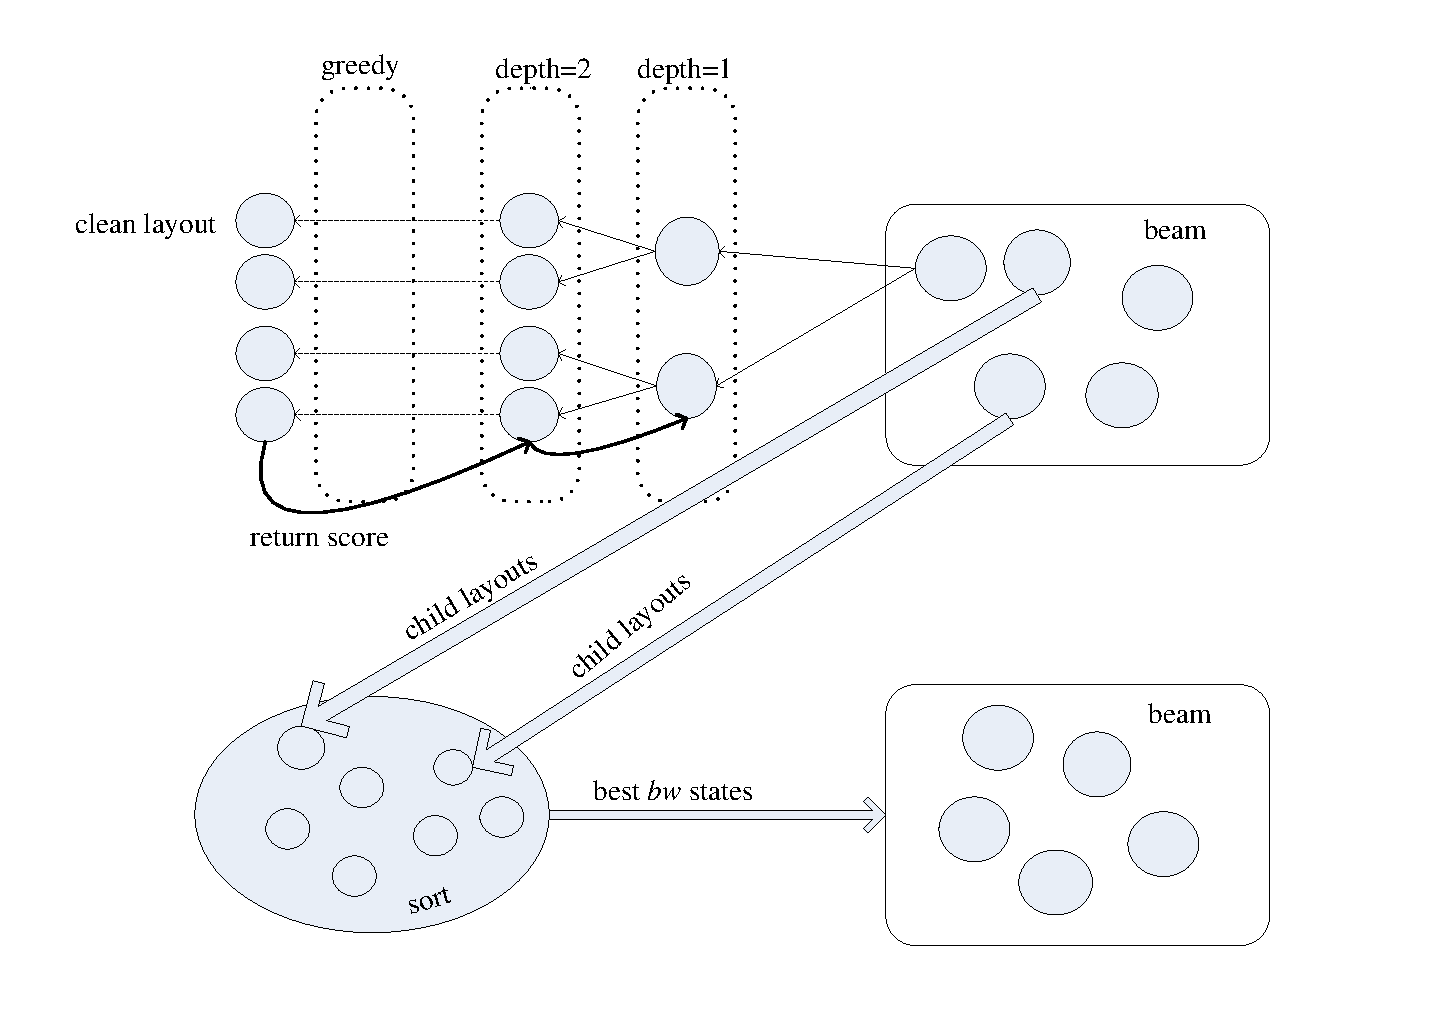
\includegraphics[width=0.4\textwidth]{fig6.pdf}
%\caption{Beam search with giant moves}
%\label{fig6}
%\end{figure*}

\begin{algorithm}[htbp]
	\caption{Beam search with giant moves for CPMP/CPMPDS}
	\label{alg:bsg}
	\begin{codebox}
	\Procname{\proc{BS-G (\id{inilay})}}
    \li $\id{beam} = \{\id{inilay}\}$
    \li \While $\id{beam} \neq \emptyset$
    \li \Do
        $\id{canlaylist}=\emptyset$
    \li \For each \id{lay} in \id{beam}
    \li     \Do
             generate up to $\id{tw}$ children of \id{lay} and append the children to \id{canlaylist}
             \End
    \li     sort the layouts in \id{canlaylist} in a descending order of scores
    \li     \id{beam} = the first $\id{bw}$ layouts in \id{canlaylist}
        \End
	\end{codebox}	
\end{algorithm}

\subsection{Beam search with baby moves}

The successor generation method of BS-G is modified to obtain another algorithm for CPMP and CPMPDS. In this algorithm, beam search is deployed to maintain the diversity of layouts; the difference from BS-G is that successors in the beam are generated by applying baby moves, hence the name beam search with baby moves~(BS-B). BS-B does not have the disadvantage of BS-G, where each giant move goes too far. Apart from the successor generation method, other components in BS-B and BS-G are the same. The process of generating successors in BS-B is as follows:

Probing tree search is applied to each layout $l$ in the beam as described in BS-G to generate \id{tw} children. The score of a child \id{chi} is the minimum score of clean offspring layouts expanded from \id{chi}. For each child $\id{chi}$ of $l$, the first interim layout on the path from $l$ to \id{chi} is recorded, and the score of this interim layout, which is the same as the score of \id{chi}, is marked. If an interim layout is the first interim layout of multiple children, the smallest score is marked. The successors of $l$ in BS-B are such interim layouts, instead of the children of $l$.

\subsection{Discussion on CPMPDS}
In this paper, three interrelated algorithms are proposed: TGH, BS-G and BS-B. These algorithms can be applied to solve CPMP and CPMPDS instances. Existing algorithms for CPMP cannot be applied directly to solve CPMPDS instances because they cannot guarantee that the dummy stack is empty when the bay is clean. If the dummy stack is ignored and a CPMPDS instance is attempted to be solved by using existing CPMP algorithms, feasible solutions may not exist because of the shortage of empty slots.
\section{Experiments and analysis}
\label{sec:ce}
The proposed algorithms are tested against the benchmark test data sets provided by \cite{BF2012} to evaluate their effectiveness.
The performance of proposed lower bounds with that of \cite{BF2012} is first compared. Then a series of experiments are conducted to evaluate the performance of the evaluation scheme and search parameters,
which is followed by the results on benchmark data.
A data set for the new CPMPDS is generated, and the result is presented for further reference. Experiments were conducted on a PC with Intel Core i7 CPU clocked at 3.40 GHz with Windows 7 operating system.

\subsection {Lower bound comparison}
Benchmark data are used to compare the performance of $\id{LB}_\id{DFS}$, $\id{LB}_\id{MKM}$, and $\id{LB}_\id{BF}$. In Table \ref{tab:lowerbound}, columns DFS, MKM, and BF indicate average lower bounds of instances in corresponding data sets calculated by $\id{LB}_\id{DFS}$, $\id{LB}_\id{MKM}$ and $\id{LB}_\id{BF}$, receptively. As such, columns tDFS, tMKM and tBF are the average computational time of three methods in seconds, which can be regarded as no difference. Table \ref{tab:lowerbound} shows that DFS and MKM have better performance than BF, but the improvement is tiny.
\begin{table}[htbp]
\centering
\caption{\label{tab:lowerbound} Lower bound comparison}
\begin{tabular}{c|c|c|c|c|c|c}
    \hline
    data set &    DFS     &     MKM   &   BF     & tDFS    & tMKM   & tBF \\
    \hline
    LC       &   29.780   &   29.659  &  29.659  & $<1$    & $<1$   & $<1$ \\
    CV       &   17.725   &   17.725  &  17.725  & $<1$    & $<1$   & $<1$ \\
    BF       &   57.239   &   57.233  &  57.231  & $<1$    & $<1$   & $<1$ \\
    \hline
    \end{tabular}%

\end{table}

\subsection {Parameter configuration}
\label{sub:config}

This section describes the experiment to evaluate the effectiveness of the evaluation scheme as well as experiments that show effect of parameters on algorithm performance. These experiments were preliminary tests performed in order to determine the final configuration of BS-G and BS-B algorithms. Data set BF is selected as test object, which is generated by \cite{BF2012} and includes 32 groups of instances, denoted by BF1, \dots, BF32; each group contains 20 instances for a total of 640 BF instances. The number of stacks in each instance is either 16 or 20, and the stack height is either 5 or 8 tiers. In addition, no dummy stack exist. The first 5 instances of each data group were tested to avoid overfitting algorithms to the benchmark data.

The effectiveness of different evaluation schemes was first investigated. Several combinations of parameters, such as probing tree width and depth and beam width, were selected to make the experiment more robust.

Three evaluation schemes were tested in the experiment. The first evaluation scheme, denoted as \texttt{smallF-ran}, is performed by evaluating candidate pairs by $f(c,s)$ plus randomness, where a random pair is selected when some pairs have the same $f$ function value. The second evaluation scheme (denoted by \texttt{smallF-lowT}) prefers small 2-tuple $(f(c,s),h(s)-\id{uf}(s))$, which are the same as the one used in TGH, BS-G and BS-B. The last evaluation scheme, denoted by \texttt{smallF-largeS}, prefers small $f(c,s)$ and large $\id{sum}$, where $\id{sum}$ is the sum of group labels of containers above the target container if the target container and stack are within the same stack; otherwise, $\id{sum}$ is the sum of group labels of containers above the target container, in conjunction with those unfixed containers in the target stack.

The above evaluation schemes were only tested on BS-G, where the probing tree width is set equal to the beam width. The result is shown in Figure \ref{fig7}. The column $w=5$ \& $d=2$ means the probing tree and beam widths are set 5 and depth is set to 2. The meanings of other columns are similar. Each bar in the chart is the average number of movements among all test instances. \texttt{smallF-lowT} has the best performance, \texttt{smallF-ran} is the second, then \texttt{smallF-largeS}. The aim of \texttt{smallF-lowT} is to fix target containers at lower tiers, whereas \texttt{smallF-largeS} aims to relocate containers with large group labels earlier. All parameter combinations show that \texttt{smallF-lowT} outperforms \texttt{smallF-largeS}, because fixing containers in lower tiers makes fixed heights among stacks even, that is, containers are fixed tier by tier to prevent containers with small group labels from occupying short stacks, and forcing the slots above them to store only dirty containers. However, relocating containers when unfixed larger groups exist is not necessary and is even considered redundant because the resulting performance is worse than that of \texttt{smallF-ran}. Thus, fixing large groups first is reasonable and effective.
\begin{figure*}[htbp]
\centering
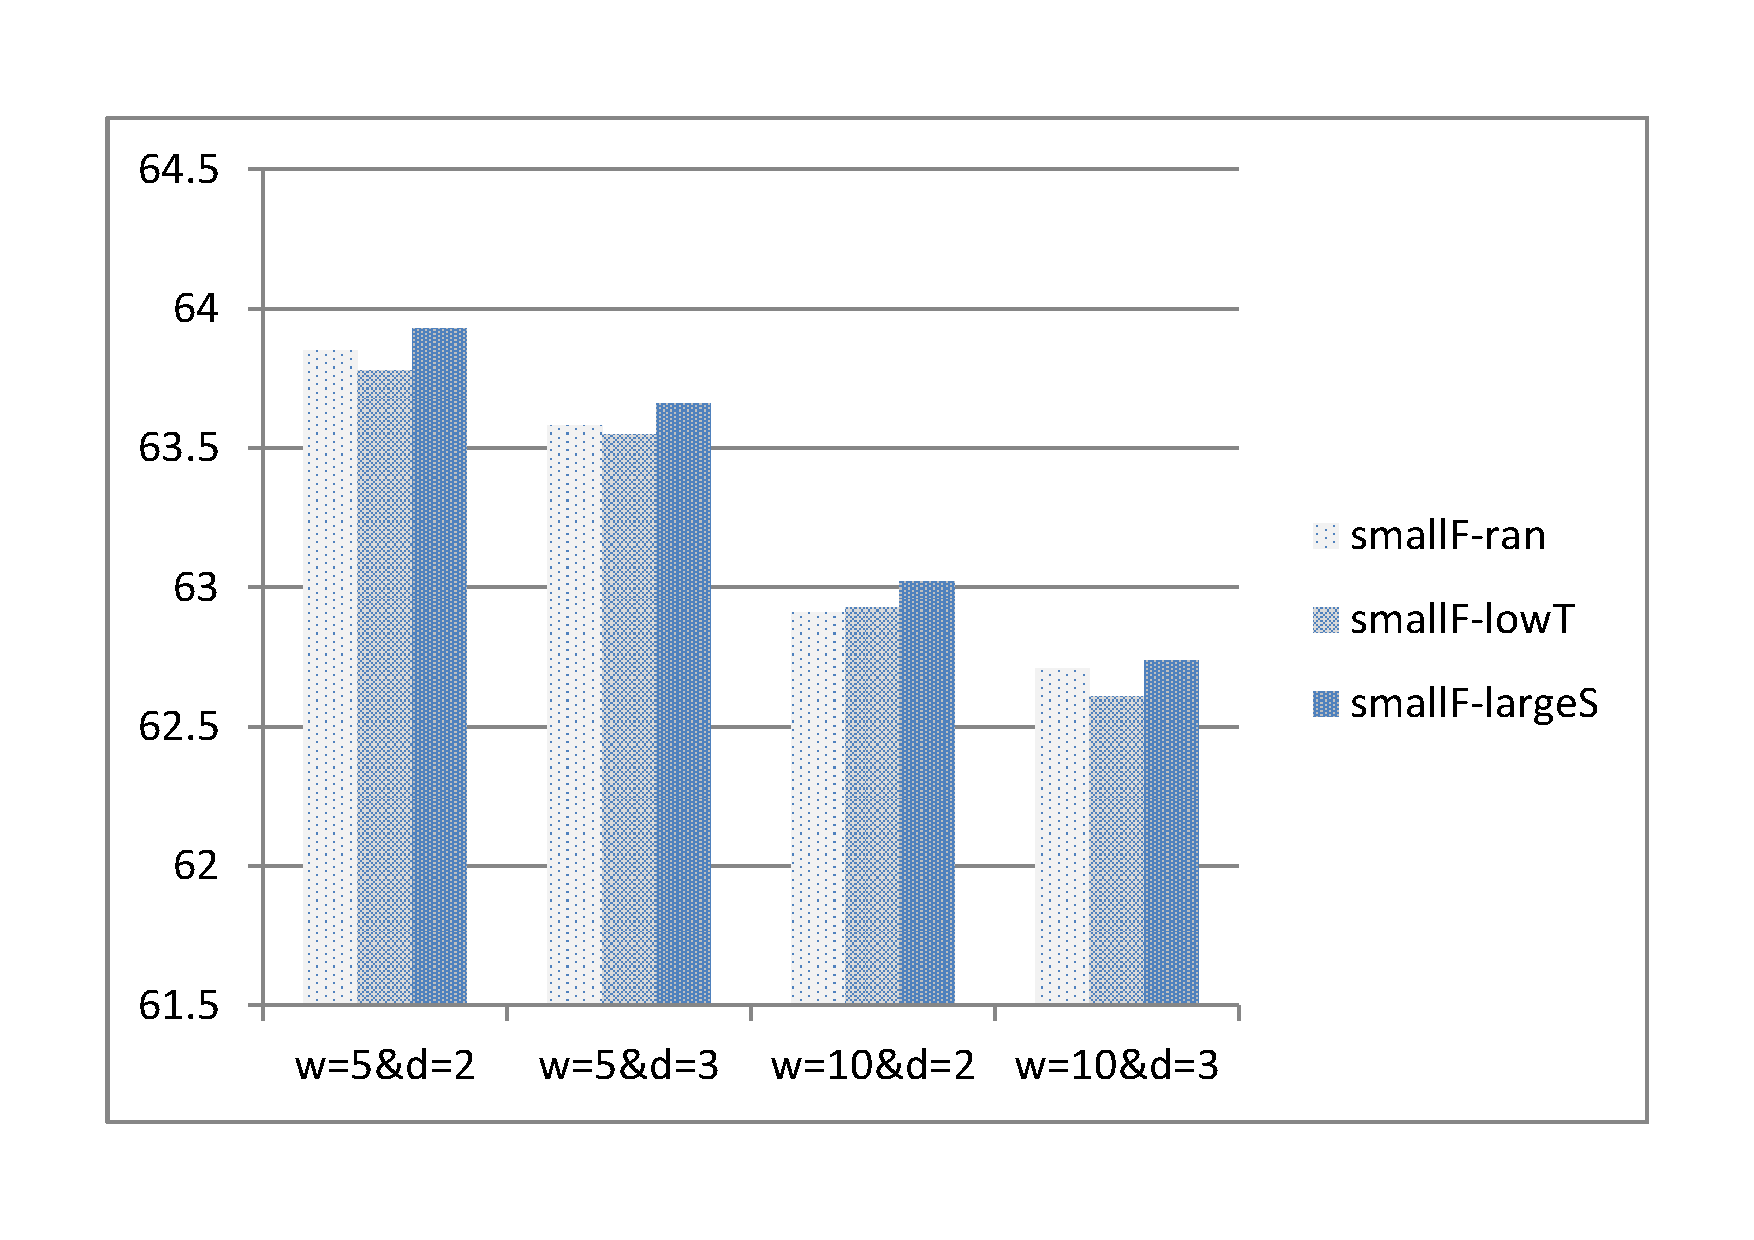
\includegraphics[width=0.4\textwidth]{fig7.pdf}
\caption{Effectiveness of evaluation schemes}
\label{fig7}
\end{figure*}
%\begin{table}[htbp]
%\centering
%\caption{\label{tab:eva_fun} Effect of evaluation function}
%\begin{tabular}{c|c|c|c|c}
%\hline
%Eva Fun      &  $w=5\&d=2$ &  $w=5\&d=3$ & $w=10\&d=2$  & $w=10\&d=3$\\
%\hline
%smallf-ran   &     63.85   &    63.58    &	  62.91     & 62.71\\
%smallf-lowt  &     63.78   &    63.55    &	  62.93     & 62.61\\
%smallf-larges&     63.93   &    63.66    &	  63.02     & 62.74 \\
%\hline
%\end{tabular}
%\end{table}



Next, the effect of probing width and depth and beam width on algorithm performance is observed. In this experiment, the evaluation scheme is set to be \texttt{smallF-lowT}. The probing tree width is set equal to the beam width, which varies from 2 to 20; $w=1$ is neglected because algorithms deteriorate to TGH when $w=1$. In addition, the computational time increases exponentially when the probing tree depth increases. Thus, the depth is only set to 1, 2, 3, or 4. BF is classified into four categories based on the number of stacks and stack height (refer to Table \ref{tab:bf}). The first category is the first eight data groups BF1$\sim$BF8 which have 16 stacks and 5 tiers in each instance. The second category is BF9$\sim$BF16 with 16 stacks and 8 tiers in each instance. The third category BF17$\sim$BF24 has 20 stacks and 5 tiers in each instance. At last, the fourth category BF25$\sim$BF32 has 20 stacks and 8 tiers in each instance.
%Again, only the first five instances of each group are tested.

The performance of BS-G on the four categories is shown separately in Figures \ref{fig8:1} to \ref{fig8:4}. Each figure shows the average number of movements of the corresponding data category obtained by BS-G for different widths and depths. The four categories have the same trend: when search width and depth increase, performance increases, but the improvement is decreasing. Furthermore, the performance of $d=2$, $d=3$ and $d=4$ are similar, which indicates that the successor generation method is considerably precise. Comparing Figures \ref{fig8:1} and \ref{fig8:2} with Figures \ref{fig8:3} and \ref{fig8:4}, the performance difference of different parameter combinations on BF1$\sim$BF8 and BF17$\sim$BF24 is tiny, whereas for BF9$\sim$BF16 and BF25$\sim$BF32, the performance difference is large. BF1$\sim$BF8 and BF17$\sim$BF24 are almost solved to the optimality even with a small depth and width (see Table \ref{tab:bf}). BF1$\sim$BF8 and BF17$\sim$BF24 are with $H=5$, whereas BF9$\sim$BF16 and BF25$\sim$BF32 are with $H=8$; all the categories have the same usage ratio. It suggests that the height limit affects instance difficulty more than the number of stacks, because containers piled vertically are harder to retrieve than those piled horizontally. %When the usage ratio equals, the instance with larger stack height is undoubtedly harder than the instance with larger stack numbers.

\begin{figure}[htbp]
\centering
\subfigure[BF1$\sim$8 average]{
    \label{fig8:1}
    \resizebox{0.4 \textwidth}{!}{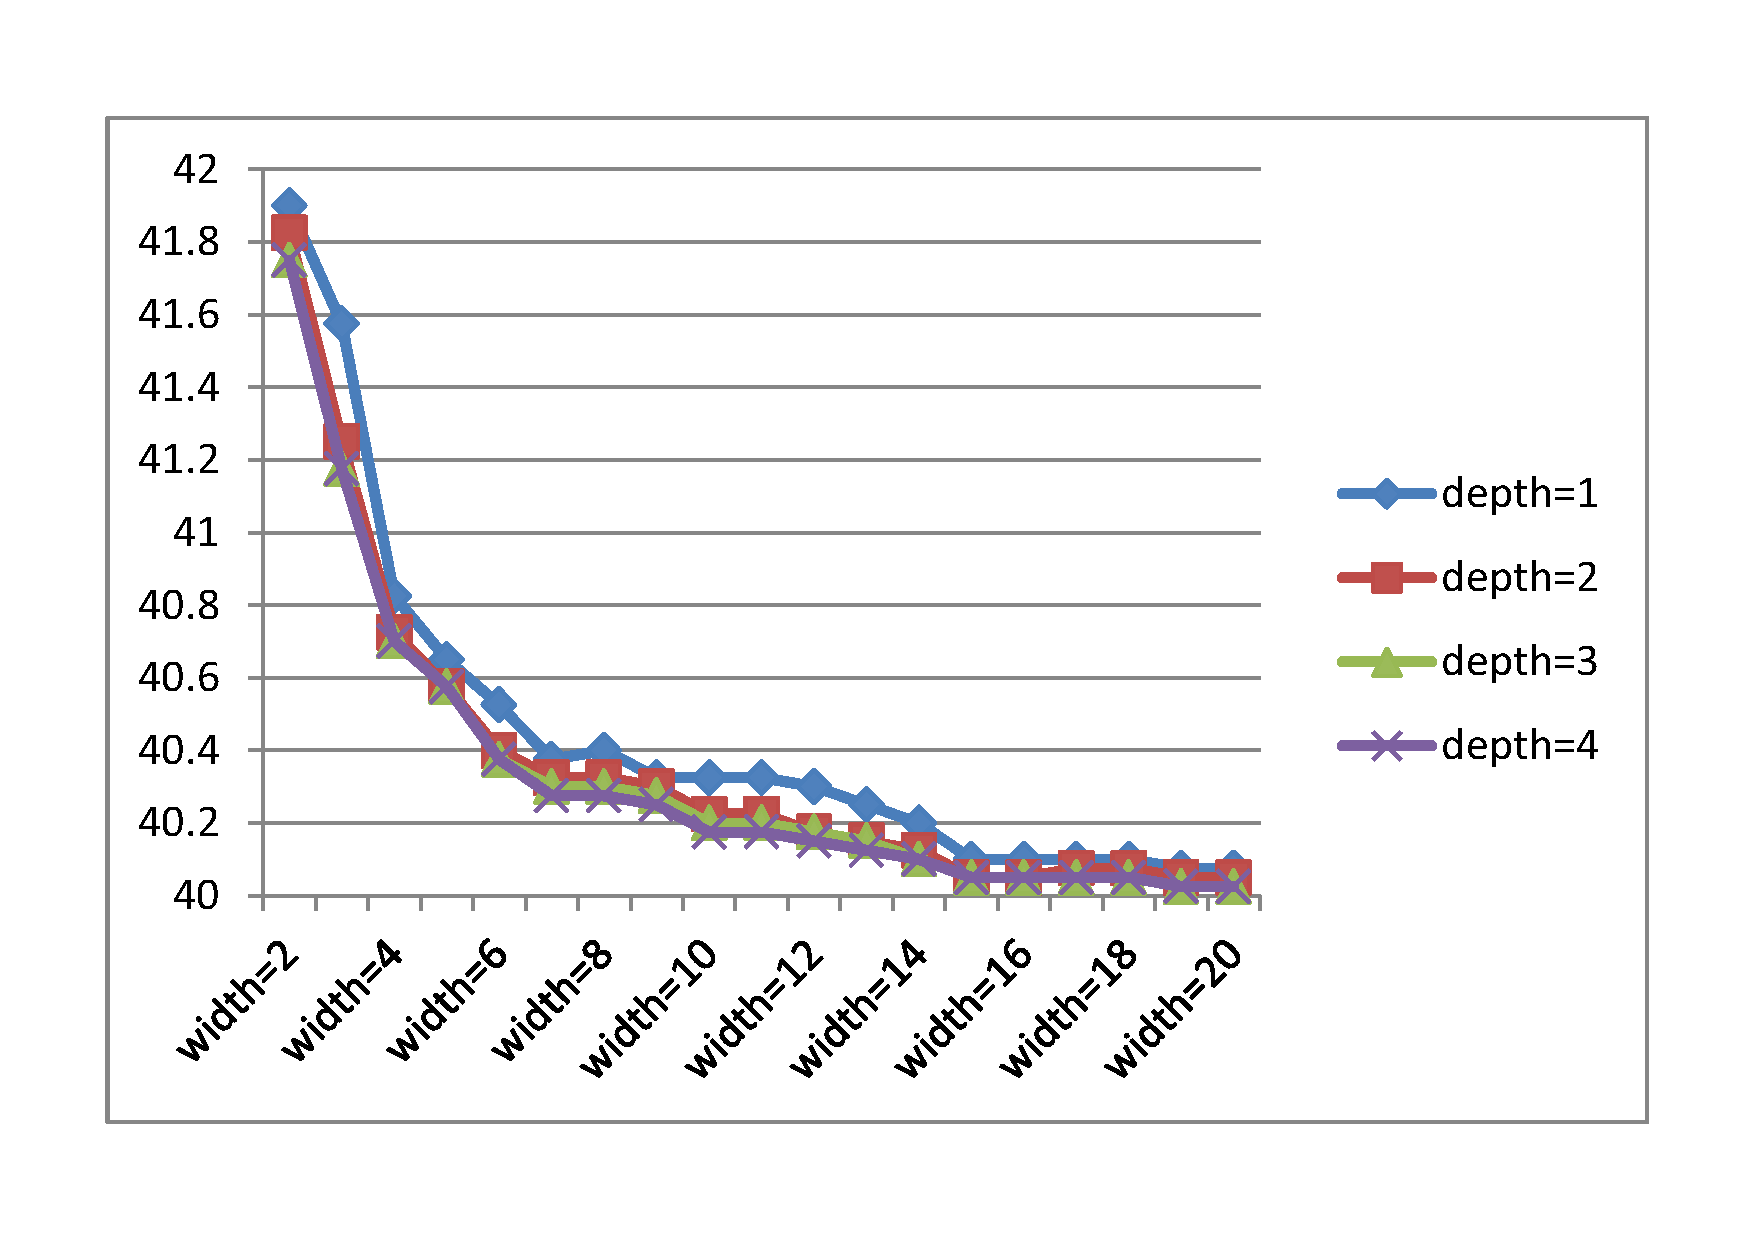
\includegraphics{fig8_1.pdf}}}
\subfigure[BF17$\sim$24 average]{
    \label{fig8:2}
    \resizebox{0.4 \textwidth}{!}{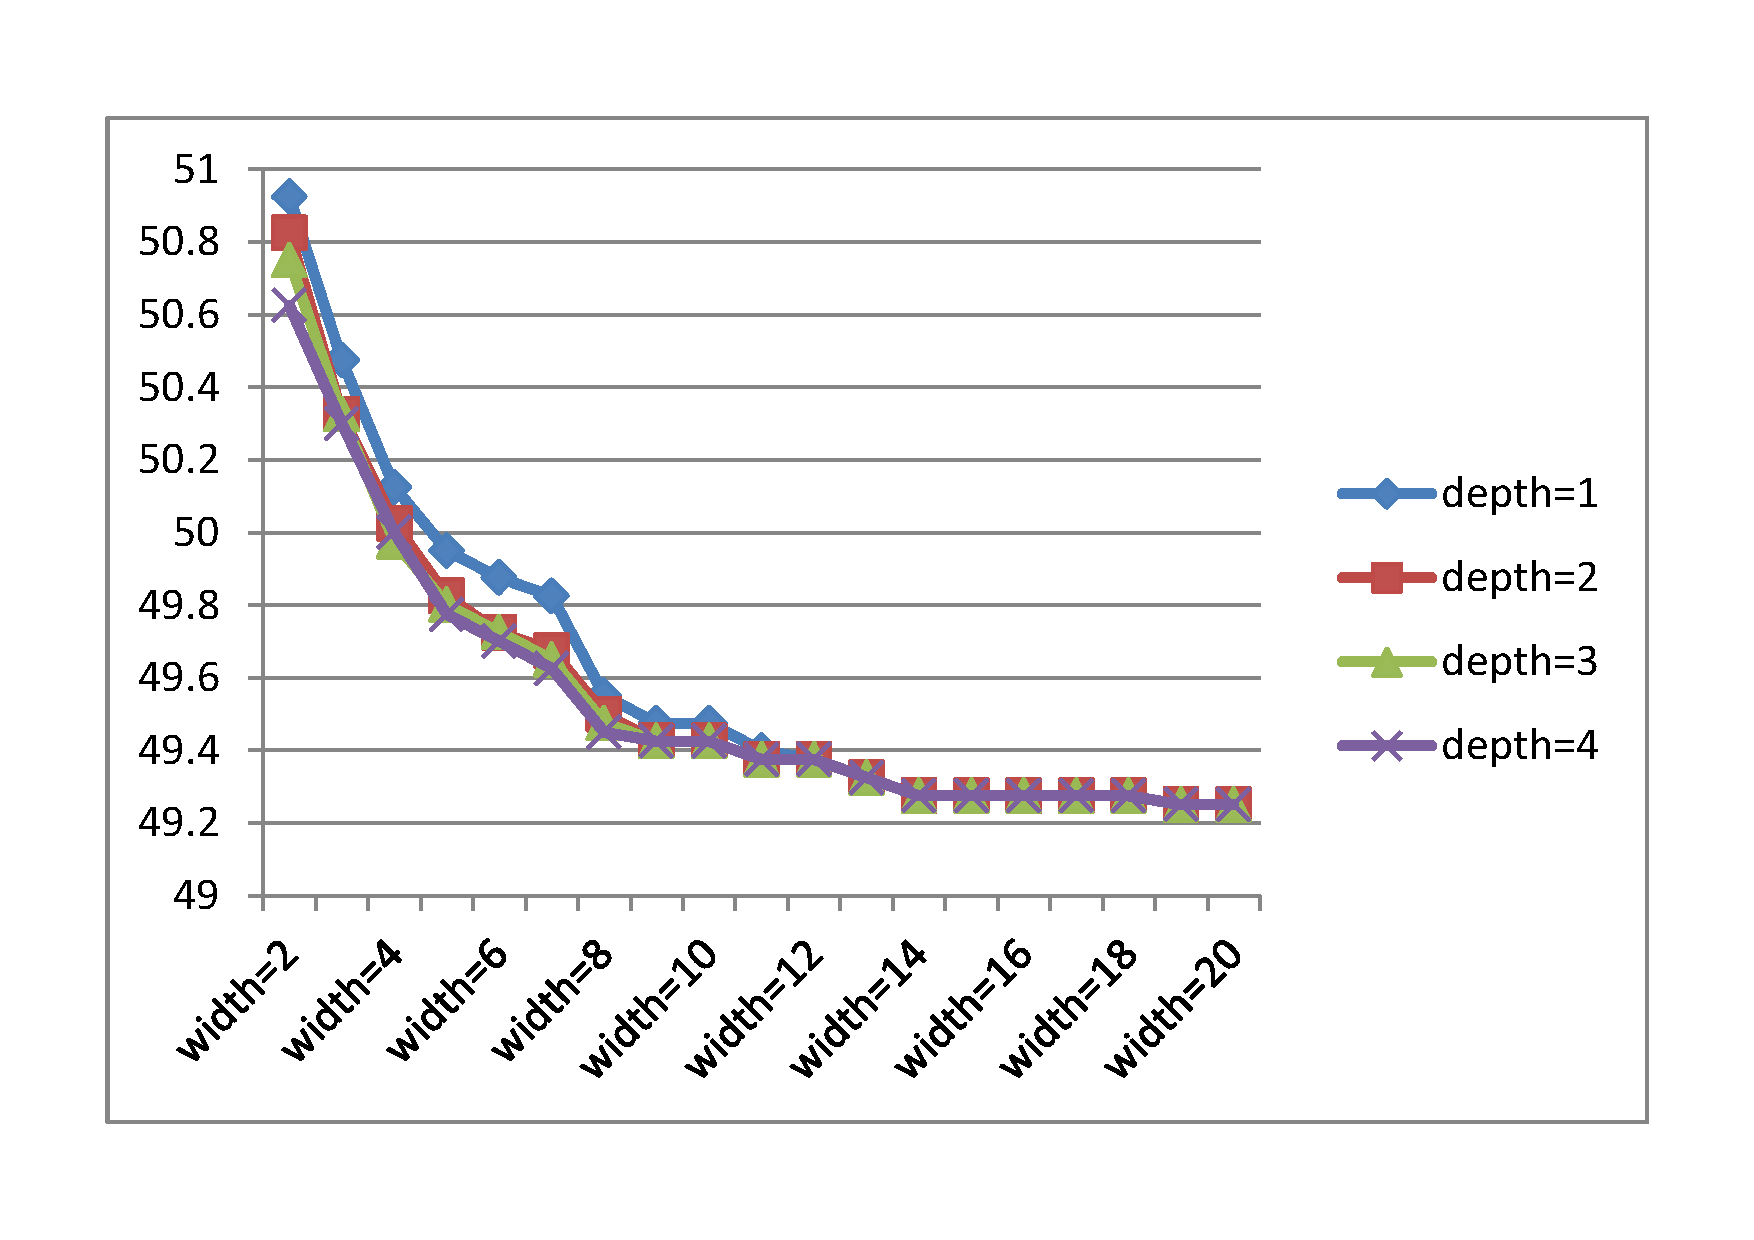
\includegraphics{fig8_2.pdf}}}
\subfigure[BF9$\sim$16 average]{
    \label{fig8:3}
    \resizebox{0.4 \textwidth}{!}{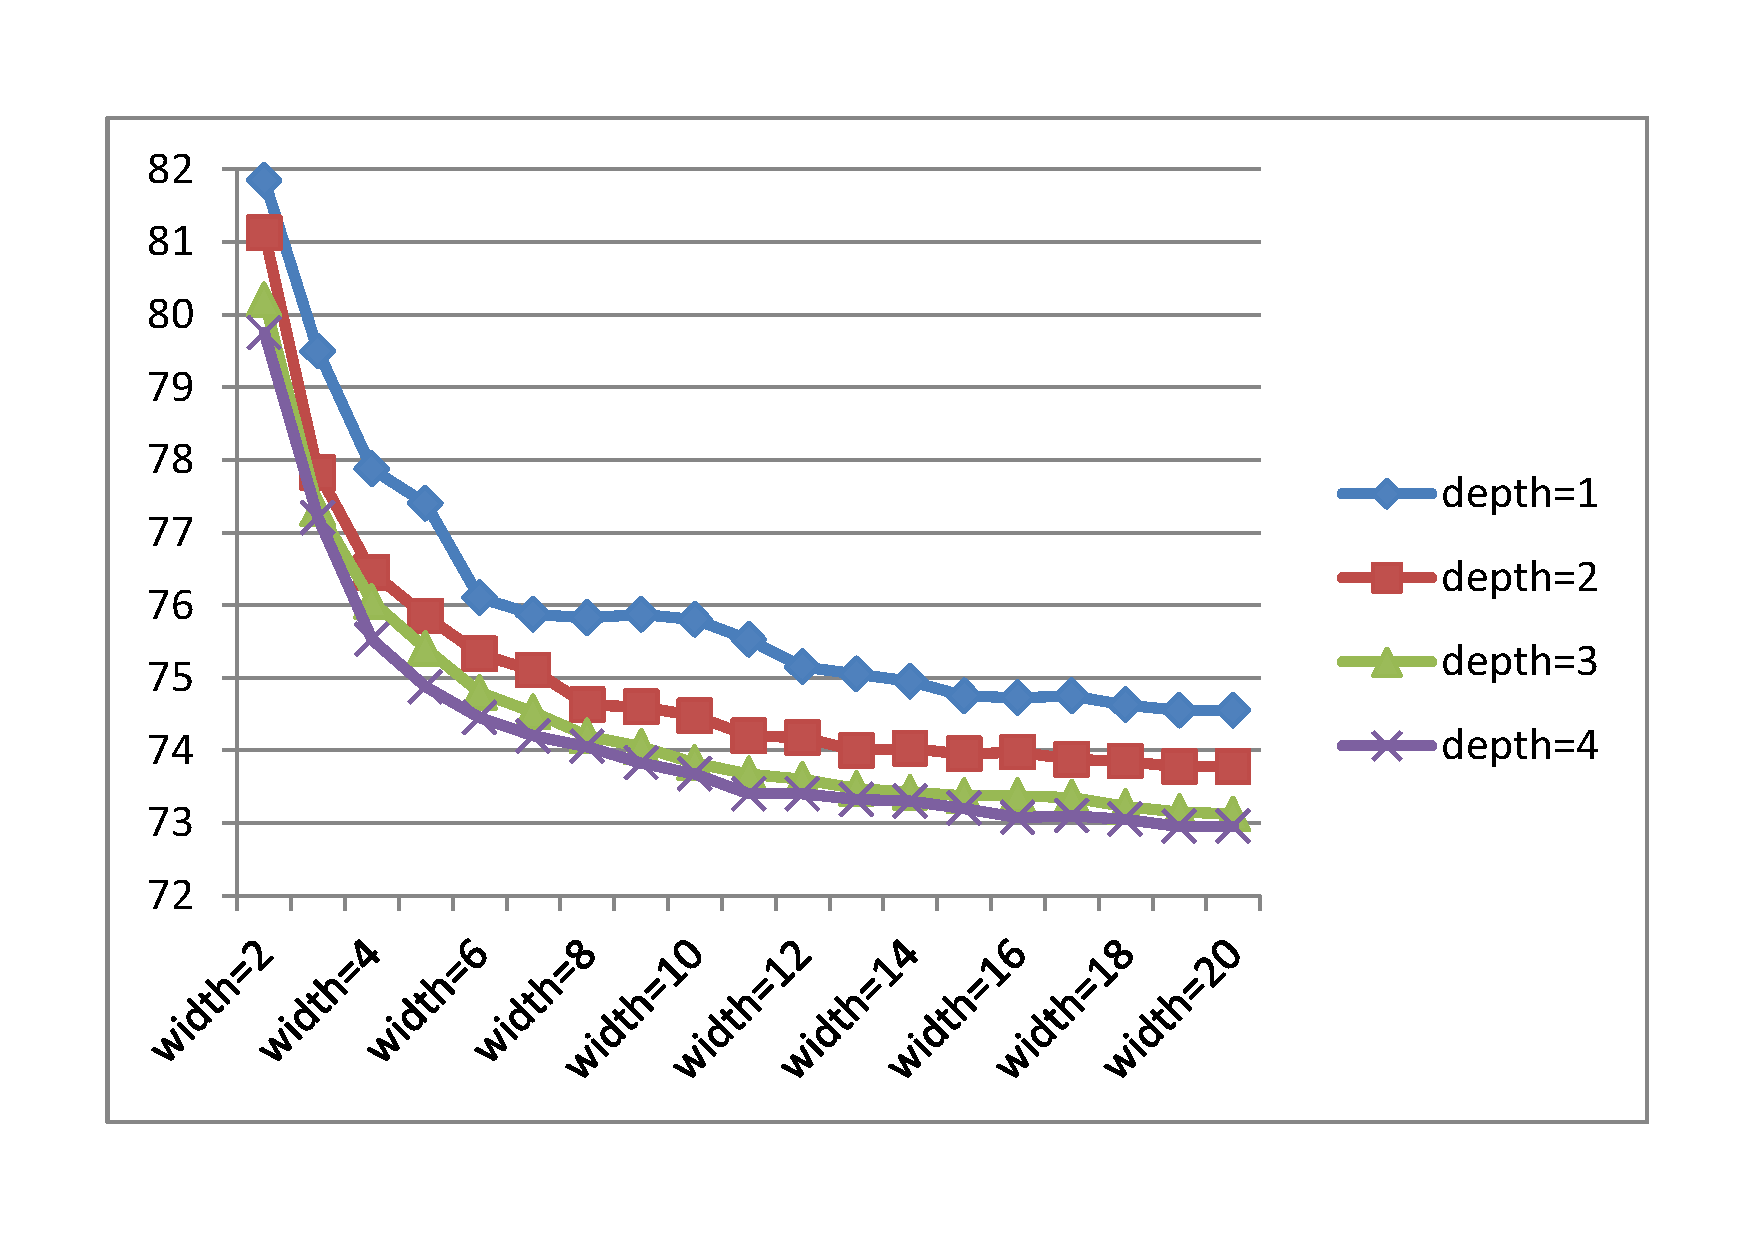
\includegraphics{fig8_3.pdf}}}
\subfigure[BF25$\sim$32 average]{
    \label{fig8:4}
    \resizebox{0.4 \textwidth}{!}{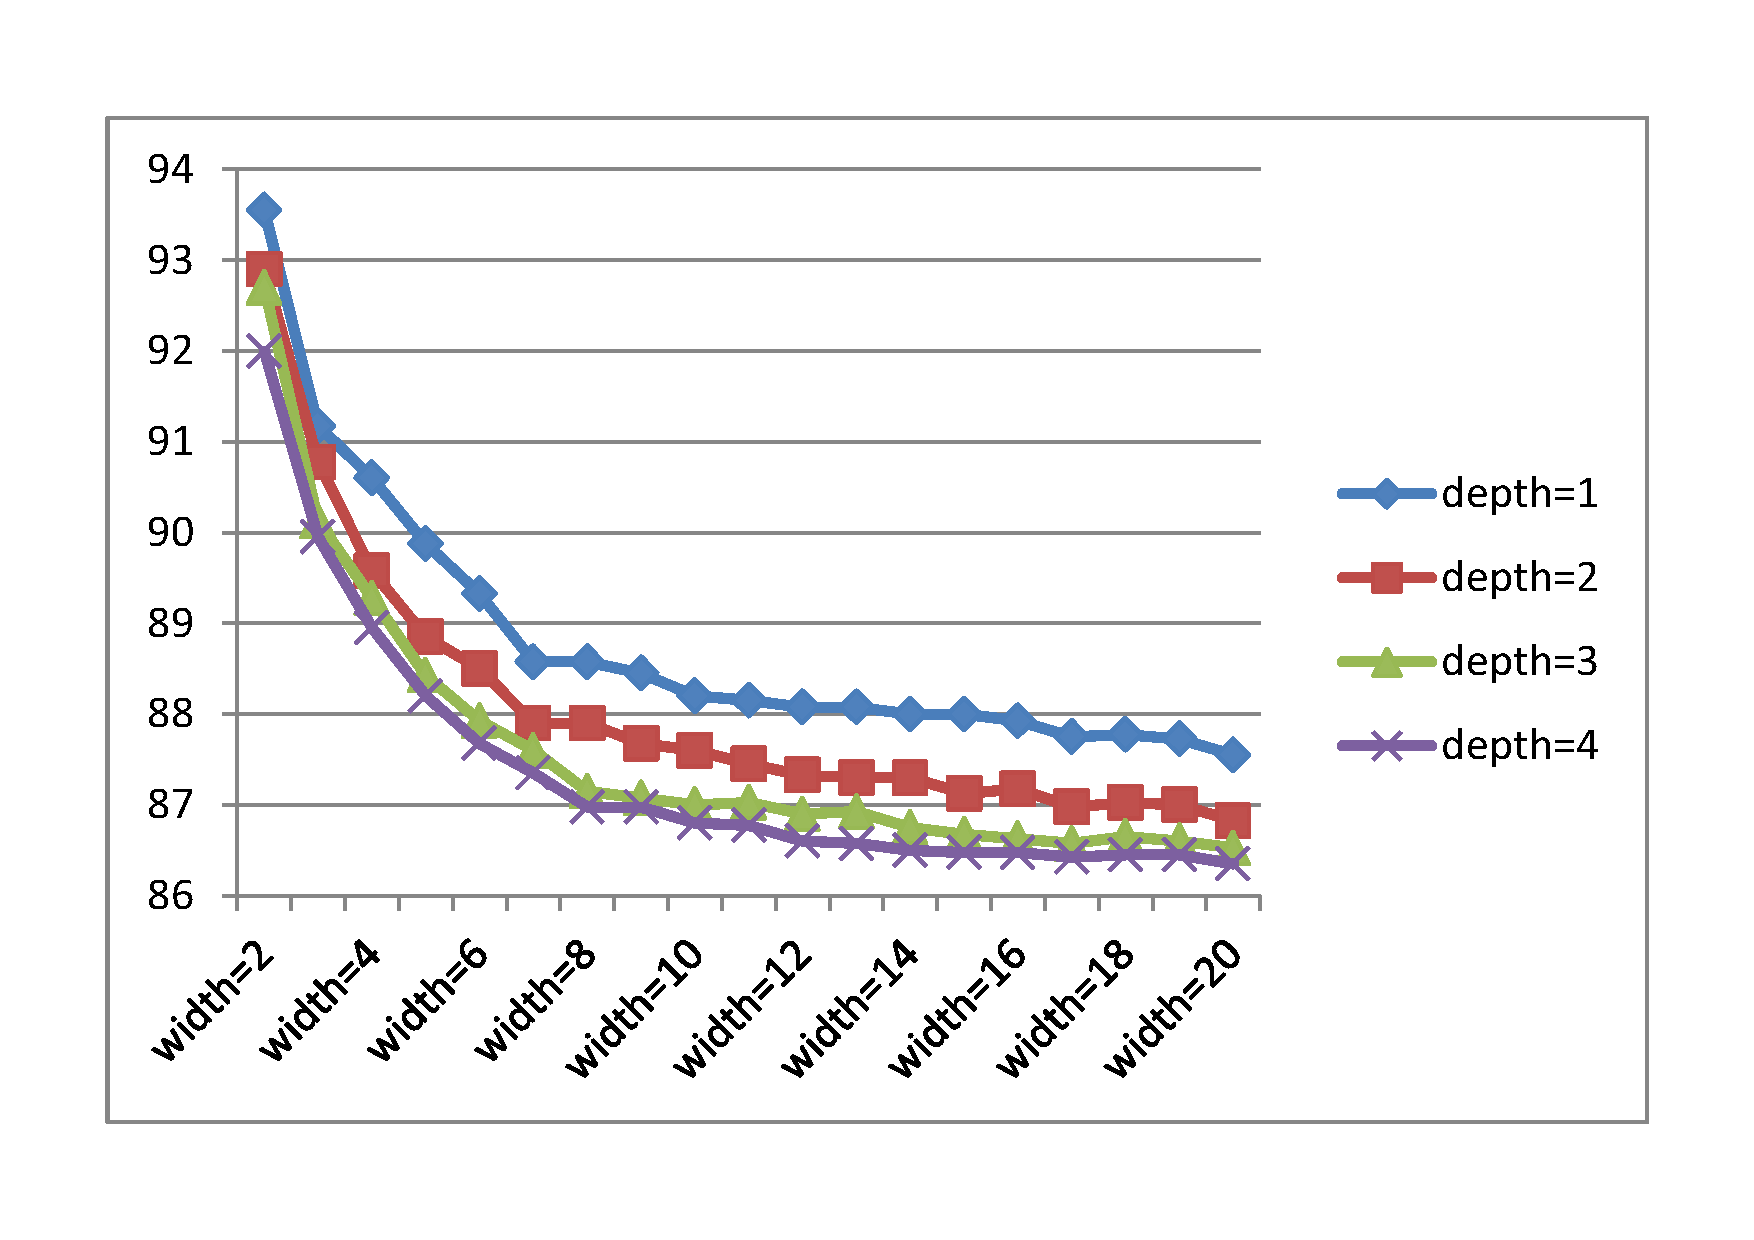
\includegraphics{fig8_4.pdf}}}
\caption{Effect of BS-G's search depth and width}
\label{fig8}
\end{figure}

The performance of BS-B on the four categories is displayed in Figure \ref{fig9}. Its trend is similar to that of BS-G in Figure \ref{fig8}; the algorithm becomes stable and the improvement decreases as parameters increase. However, the performance sometimes returns to a larger value as width increase, especially when the depth is small. For example, in Figure \ref{fig9:4}, the performance when $w=8$ \& $d=1$ is better than the performance when $w=10$ \& $d=1$. The explanation is the algorithm degenerates to evaluate successors by TGH when $d=1$. A smaller depth leads to a weaker ability of BS-B to evaluate successors; therefore, performance deterioration is observed. When the search depth increases, performance deterioration disappears. This phenomenon indicates that heuristic TGH alone is not enough to evaluate successors precisely and incorporating probing tree search is necessary.
\begin{figure}[htbp]
\centering
\subfigure[BF1$\sim$8 average]{
    \label{fig9:1}
    \resizebox{0.4 \textwidth}{!}{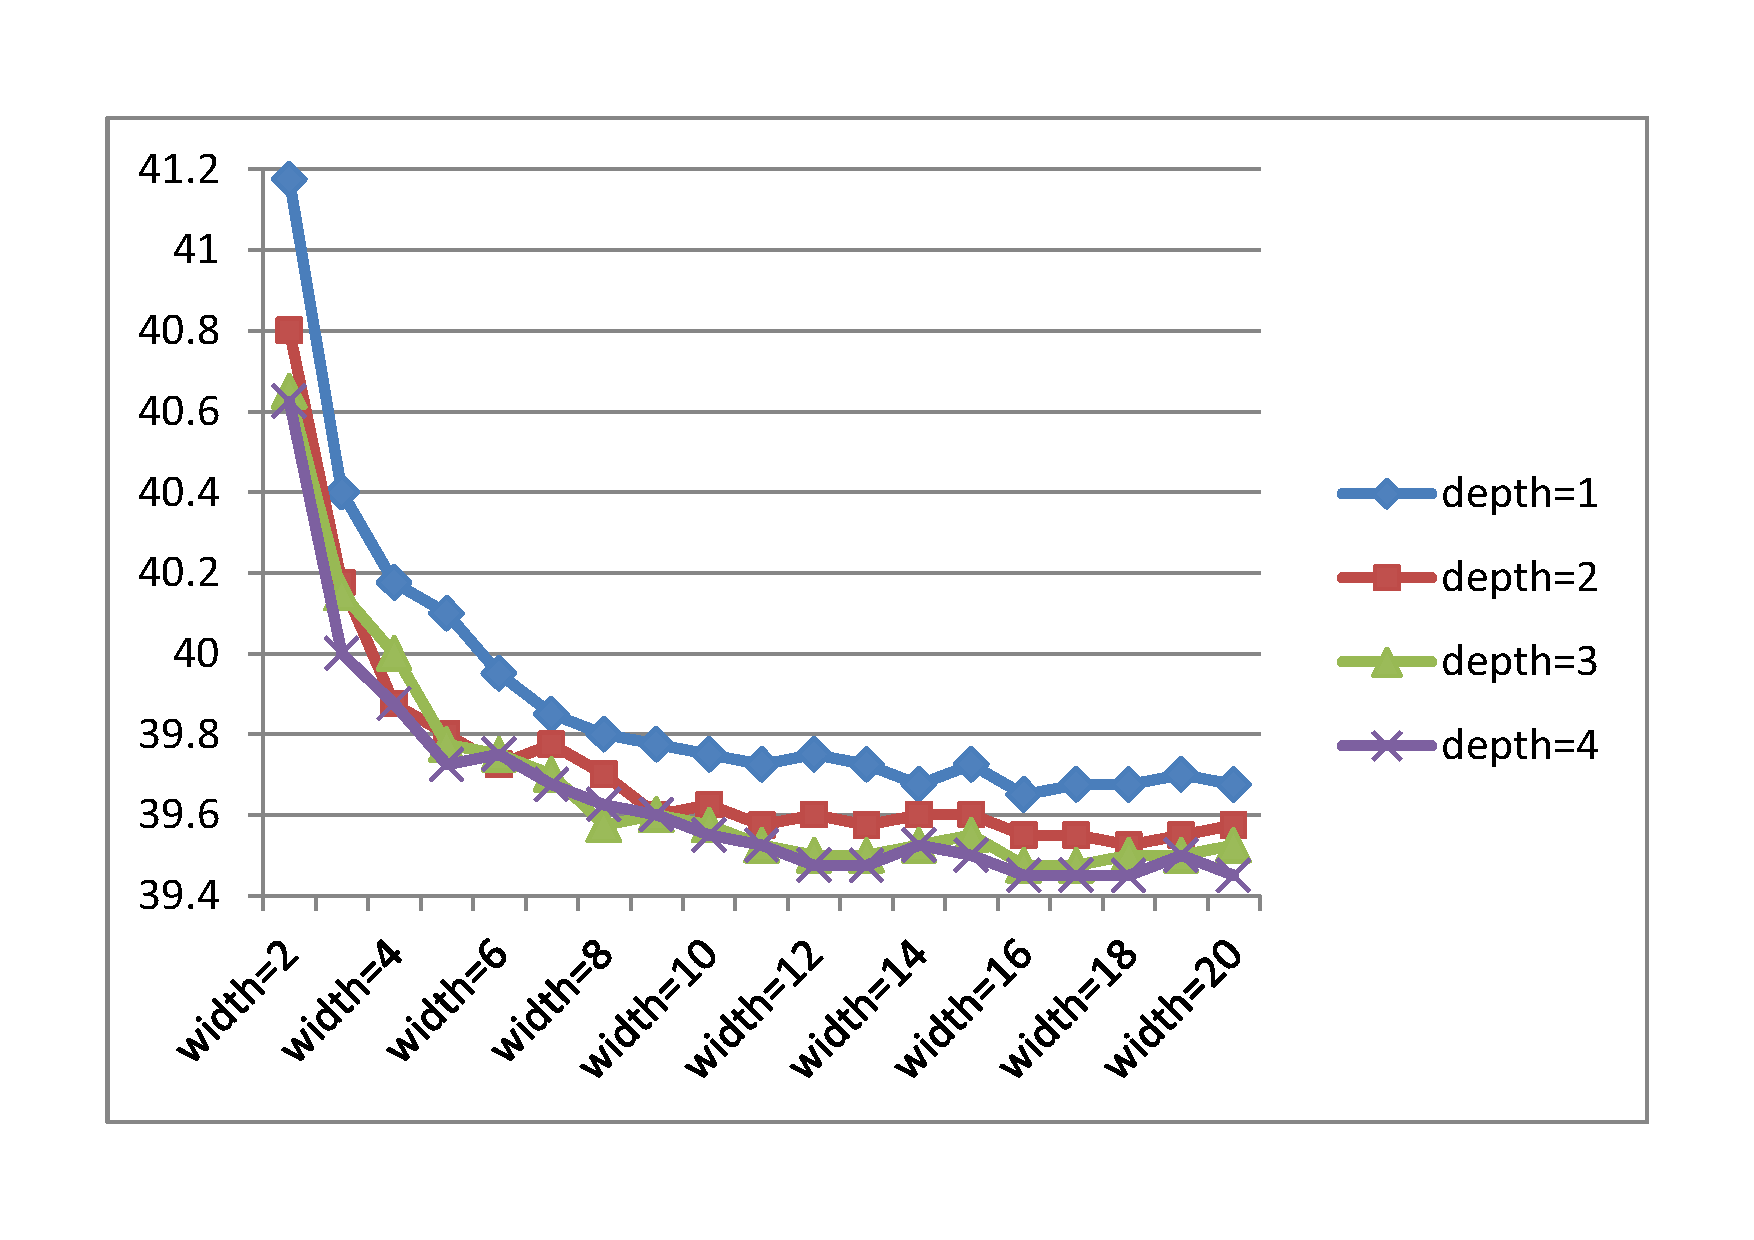
\includegraphics{fig9_1.pdf}}}
\subfigure[BF17$\sim$24 average]{
    \label{fig9:2}
    \resizebox{0.4 \textwidth}{!}{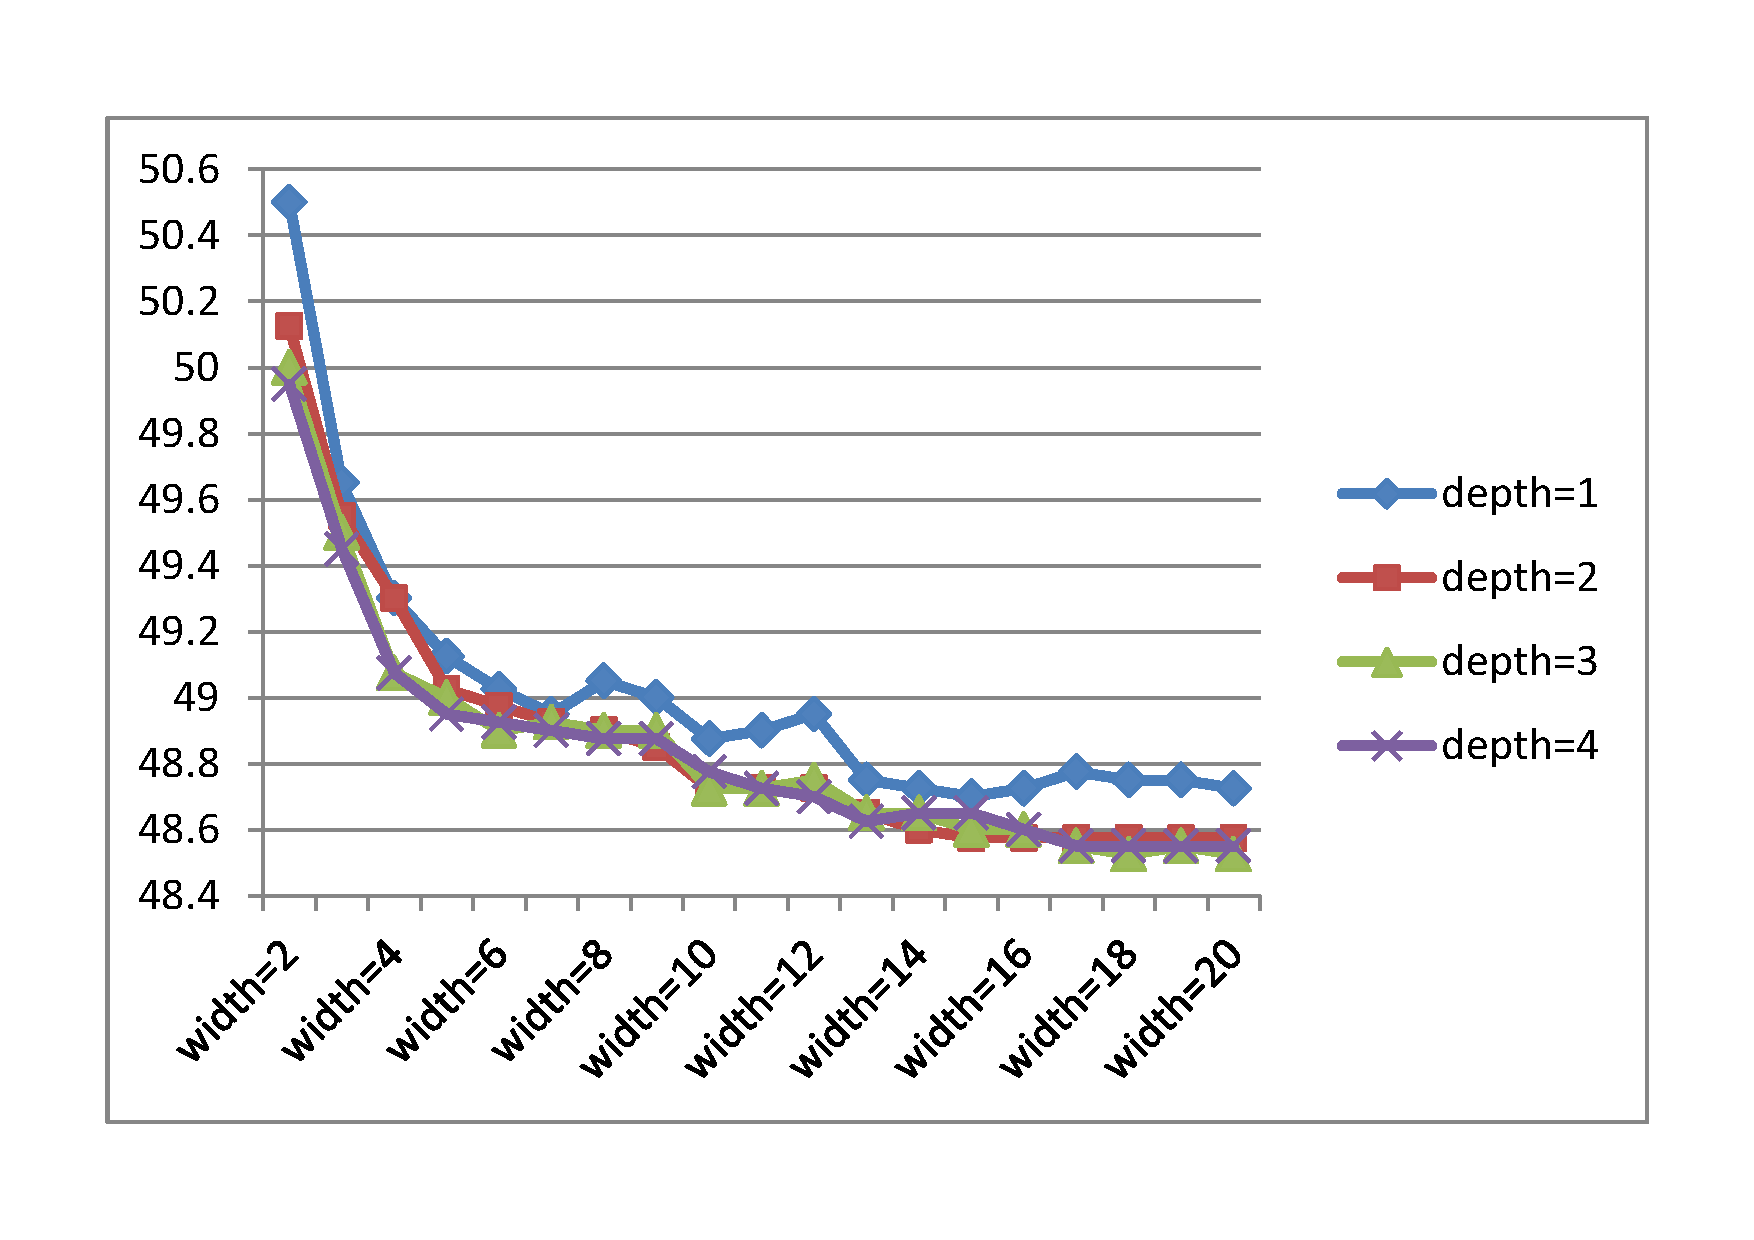
\includegraphics{fig9_2.pdf}}}
\subfigure[BF9$\sim$16 average]{
    \label{fig9:3}
    \resizebox{0.4 \textwidth}{!}{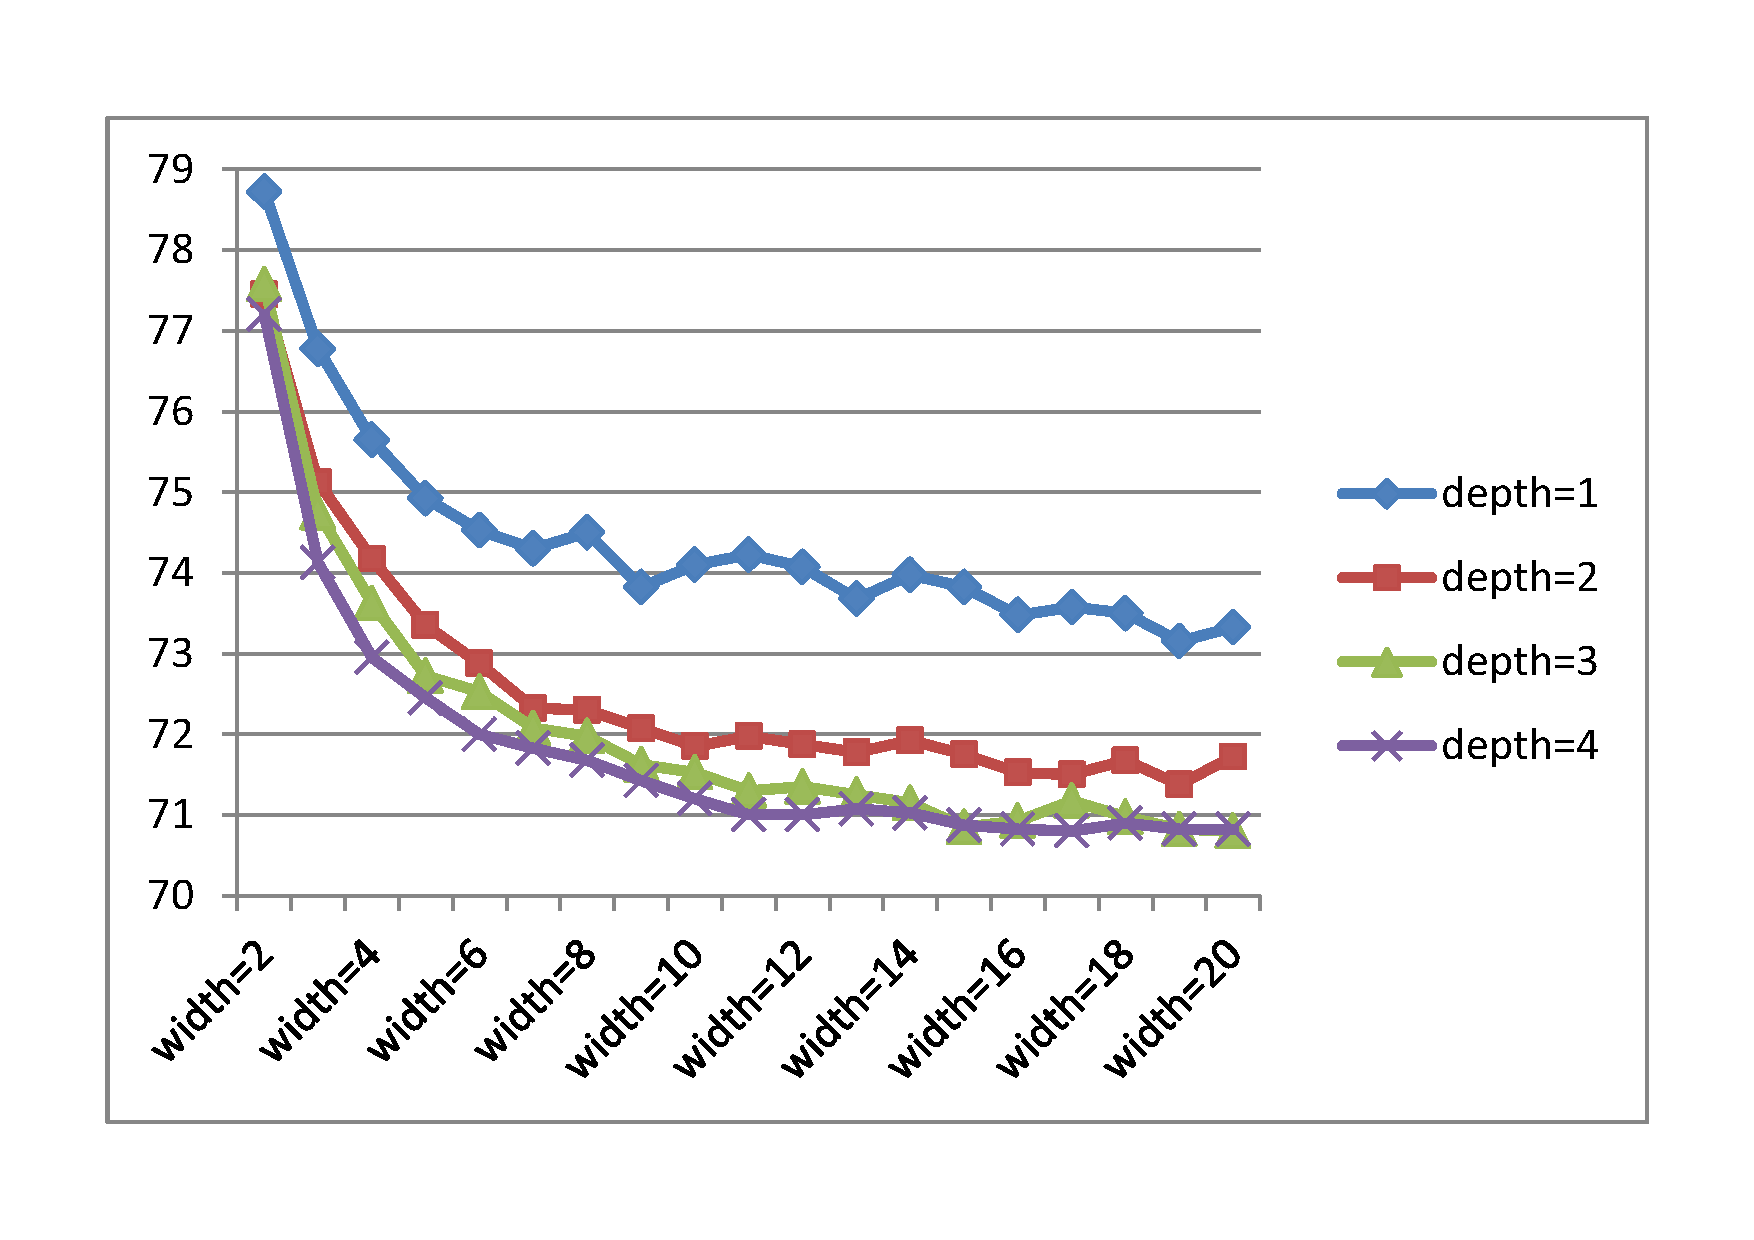
\includegraphics{fig9_3.pdf}}}
\subfigure[BF25$\sim$32 average]{
    \label{fig9:4}
    \resizebox{0.4 \textwidth}{!}{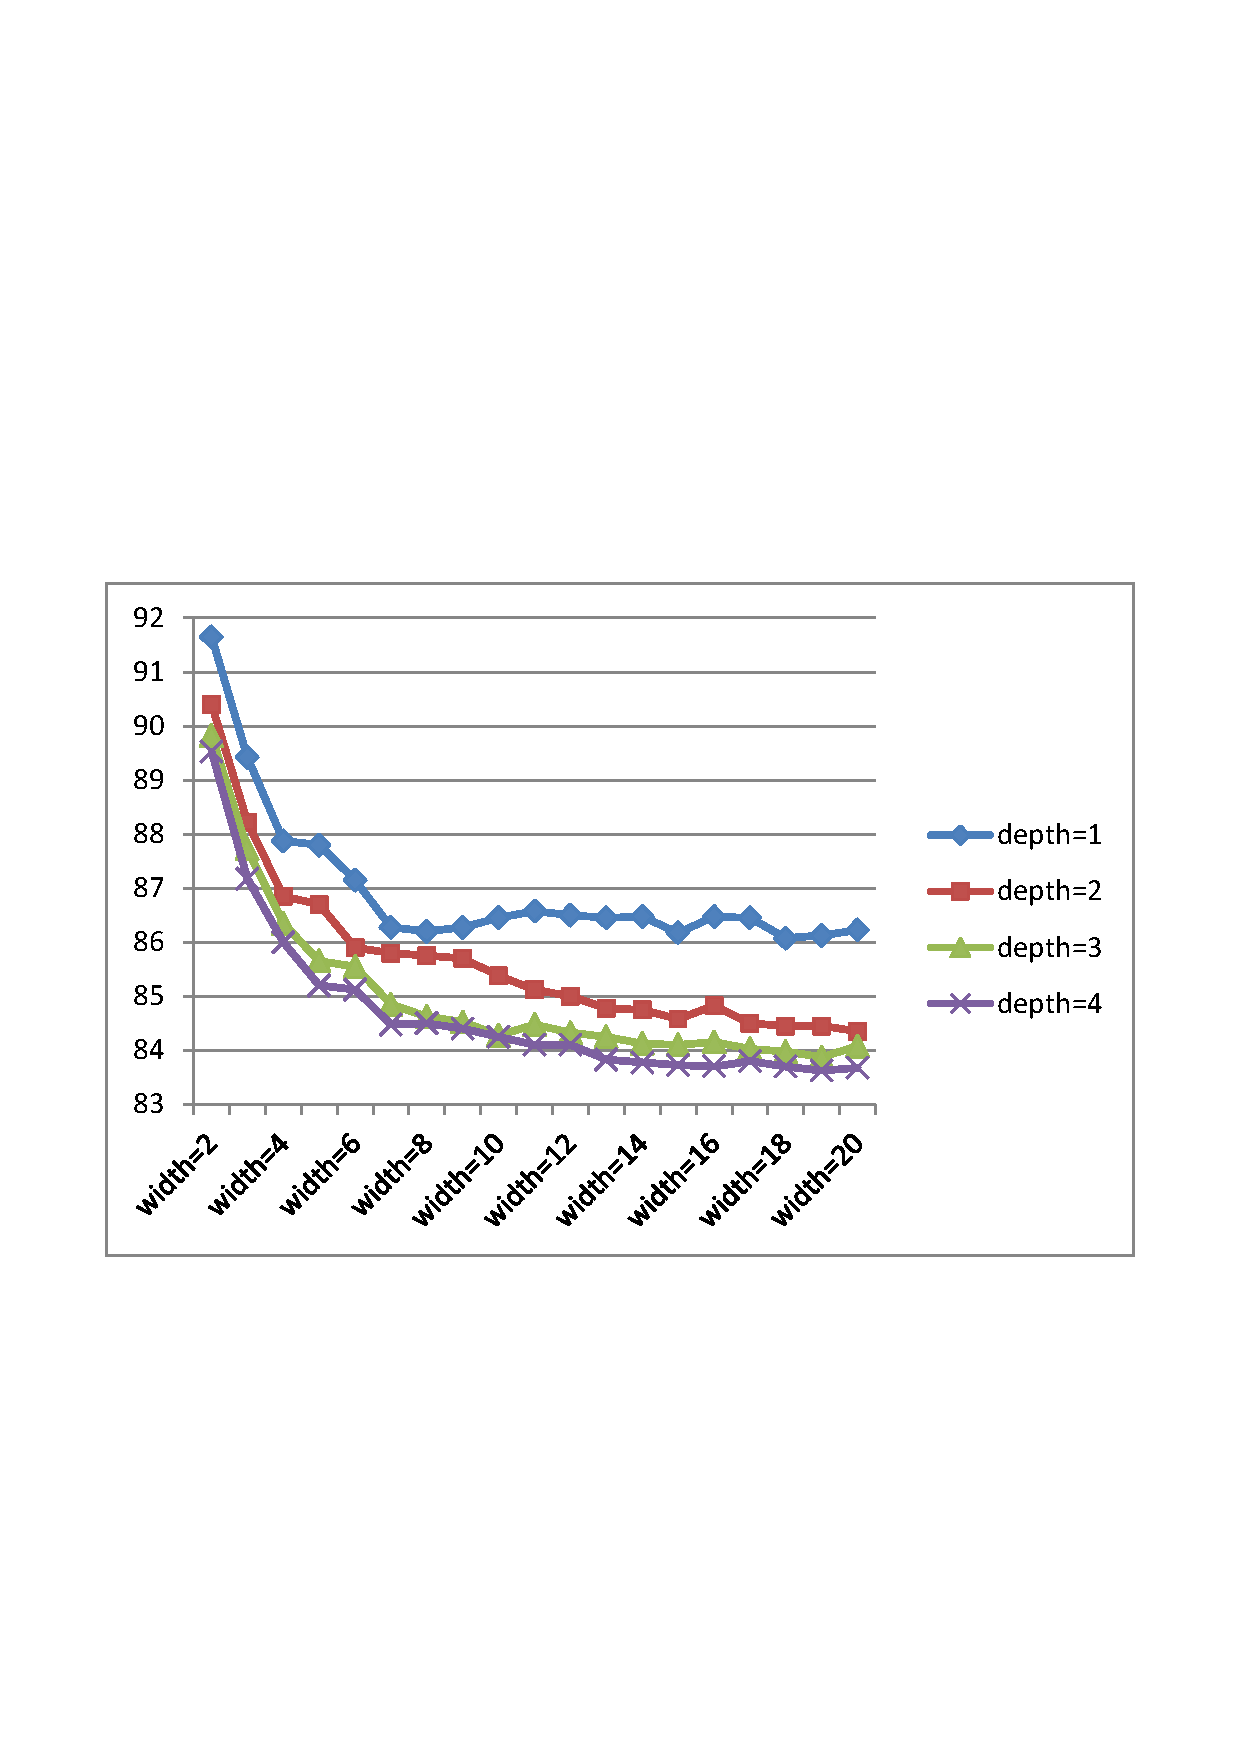
\includegraphics{fig9_4.pdf}}}
\caption{Effect of BS-B's search depth and width}
\label{fig9}
\end{figure}

\subsection {Comparison with existing approach}

The proposed algorithms were compared with the tree search algorithm by \cite{BF2012} (hereafter BF2012 for short) on CPMP benchmark data. BF2012 has the best performance on CPMP. The environment of BF2012 is Intel Core 2 Duo processor (P7350, 16 GFLOPS) with 2 GHz and 2 GB RAM under Mac OS X and code was written in C and compiled with XCode under Mac OS X. In the algorithms proposed in this paper, parameters of BS-G and BS-B are set to $\id{bw}=\id{tw}=20$ and $\id{td}=3$, since BS-G and BS-B become stable and the improvement is negligible if parameters increase, as shown in Figure \ref{fig8} and Figure \ref{fig9}. 

To begin with, the result of data set LC mentioned in Section 7.2 of \cite{BF2012} is shown. LC is first generated by \cite{Lee2009}, but the concrete data set is not available. Hence, \cite{BF2012} generated a new set of instances according to the description of \cite{Lee2009}. The result of LC is shown in Table \ref{tab:lc}, where the first five columns summarize data information copied from \cite{BF2012}. The dirty ratio is the number of dirty containers in the initial layout divided by the number of total containers.
Columns BF2012, TGH, BS-G and BS-B are the average movements on each data group by the respective algorithms. The average run time in seconds by BF2012, BS-G and BS-B is reported in columns tBF2012, tBS-G and tBS-B, respectively. The run time of TGH is omitted from the table because it is less than 0.2s. Column $\id{LB}_\id{DFS}$ indicates the average lower bounds $\id{LB}_\id{DFS}$ on each data group and column gap is the gap between BS-B and $\id{LB}_\id{DFS}$. The last row of the table shows the mean number of movements on LC. When calculating average time, times with ``$<1$''  and ``$<0.1$" are regarded as 1 and 0.1 s, respectively. Those results that our algorithms outperform BF2012 are highlighted in bold. Algorithms TGH and BS-G are worse than BF2012, whereas BS-B is better than BF2012. However, the improvement is minimal,because the size of test instances is too small and BF2012 has almost solved the instances to the optimality, which can be inferred from the absolute spread between lower bounds and solutions.
\begin{table}[htbp]
\scriptsize
\centering
  \caption{\label{tab:lc} Comparison of LC data}
    \begin{tabular}{c|c|c|c|c|c|c|c|c|c|c|c|c|c}

    \hline
    group & stack & height & usage rate & dirty ratio & BF2012 & tBF2012 & TGH   & BS-G  & tBS-G & BS-B  & tBS-B & $\id{LB}_\id{DFS}$ & gap\\
    \hline
    LC1   & 10   & 5  & 0.7  & 0.37 & 17   & $<1$ & 22   & 17         & $<0.1$ & 17             & $<1$  & 15 & 13.33\%\\
    LC2a  & 12   & 6  & 0.69 & 0.38 & 22.6 & 1    & 26.9 & 23.2       & $<0.1$ & \textbf{22.3}  & $<1$  & 21.1 & 5.69\%\\
    LC2b  & 12   & 6  & 0.69 & 0.7  & 38.4 & 2.1  & 46.7 & \textbf{38}& $<0.1$ & \textbf{37.9}  & 1.37  & 37.3 & 1.61\%\\
    LC3a  & 12   & 6  & 0.75 & 0.39 & 23.7 & 1.4  & 29.1 & 23.9       & $<0.1$ & 23.7           & $<1$  & 22.3 & 6.28\%\\
    LC3b  & 12   & 6  & 0.75 & 0.67 & 42.7 & 4.2  & 54.8 & 43.6       & $<1$   & \textbf{42.3}  & 10.33 & 39.9 & 6.02\%\\
    \hline
    Ave   & 11.6 & 5.8& 0.72 & 0.5  & 28.88& 1.94 & 35.9 & 29.14      & $<1$   & \textbf{28.64} & 2.69  & 27.12&
    5.6\% \\
    \hline
    \end{tabular}%
\end{table}%

Then the proposed algorithms were compared with BF2012 on data set CV. CV is provided by \cite{Caserta2009} and \cite{BF2012} has the best performance on it. Table \ref{tab:cv} illustrates the comparative result that both BS-G and BS-B surpass BF2012.
\begin{table}[htbp]
\scriptsize
  \centering
  \caption{\label{tab:cv} Comparison of CV data}
    \begin{tabular}{c|c|c|c|c|c|c|c|c|c|c|c|c|c}
    \hline
    group & stack & height & usage rate & dirty ratio & BF2012 & tBF2012 & TGH   & BS-G  & tBS-G & BS-B  & tBS-B & $\id{LB}_\id{DFS}$ & gap\\
    \hline
    CV1  & 3  & 9   & 0.33 & 0.6  & 10.5 & $<1$ & 12.1 & 10.6          & $<0.01$ & \textbf{10}   & $<0.01$ &7.9 & 26.58\%\\
    CV2  & 4  & 16  & 0.25 & 0.66 & 19.1 & $<1$ & 20.3 & \textbf{17.8} & $<0.01$ & \textbf{17.2} & $<0.1$ &13.6 & 26.47\%\\
    CV3  & 5  & 25  & 0.2  & 0.7  & 30.4 & 9.1  & 34   & \textbf{27.3} & $<0.1$  & \textbf{26.4} & $<1$   &21.3 & 23.94\%\\
    CV4  & 6  & 36  & 0.17 & 0.74 & 44.4 & 20   & 50   & \textbf{37.1} & $<0.1$  & \textbf{35.9} & $<1$   &28.1 & 27.76\%\\
    \hline
    Ave  & 4.5& 21.5& 0.24 & 0.67 & 26.1 & 7.78 & 29.1 & \textbf{23.2} & $<0.1$  & \textbf{22.38}& $<1$   & 17.73 & 26.23\%\\
    \hline
    \end{tabular}%
\end{table}%

Finally, the result of data set BF is shown in Table \ref{tab:bf}. BF is generated by \cite{BF2012}; the produced instances are supposedly difficult enough to justify the performance of algorithms. The performance of TGH is worse than that of BF2012, because BF2012 deploys a tree search algorithm, whereas TGH is only a greedy heuristic. BS-G and BS-B outperform BF2012 by almost 5\% and 7\%, respectively. 
%What's more, the computational time of BS-G is less than that of BF2012. Although the computational time of BS-B is much more than that of BF2012 in Table \ref{tab:bf}, the results are still better than that of BF2012 if we decrease parameters to make run the time of BS-B close to the run time of BF2012.

\begin{table}[htbp]
\caption{\label{tab:bf} Comparison of BF data}
\scriptsize
\begin{tabular}{c|c|c|c|c|c|c|c|c|c|c|c|c|c}
  \hline
  group & stack & height & usage rate & dirty ratio & BF2012 & tBF2012 & TGH   & BS-G  & tBS-G & BS-B  & tBS-B & $\id{LB}_\id{DFS}$ & gap\\
    \hline
    BF1   & 16 & 5  & 0.6 & 0.6  & 29.1  & $<1$  & 29.1   & 29.1          & $<0.01$ & 29.1           & $<0.01$ & 29.1  & 0\\
    BF2   & 16 & 5  & 0.6 & 0.75 & 36    & $<1$  & 36     & 36            & $<0.01$ & 36             & $<0.01$ & 36    & 0\\
    BF3   & 16 & 5  & 0.6 & 0.6  & 29.1  & $<1$  & 29.45  & 29.15         & $<0.01$ & 29.1           & $<0.1$  & 29.1  & 0\\
    BF4   & 16 & 5  & 0.6 & 0.75 & 36    & $<1$  & 36     & 36            & $<0.01$ & 36             & $<0.01$ & 36    & 0\\
    BF5   & 16 & 5  & 0.8 & 0.61 & 41.6  & 8     & 48.25  & 42.05         & $<0.1$  & \textbf{41.35} & 3.73    & 40.75 & 1.47\%\\
    BF6   & 16 & 5  & 0.8 & 0.75 & 49.4  & 4.9   & 57.65  & 51.1          & $<0.1$  & 50.15          & 10.87   & 48.6  & 3.19\%\\
    BF7   & 16 & 5  & 0.8 & 0.61 & 42.9  & 26.3  & 53.5   & 44.75         & $<0.1$  & 43.05          & 8.95    & 41.3  & 4.24\%\\
    BF8   & 16 & 5  & 0.8 & 0.75 & 50.6  & 24.7  & 60.05  & 51.95         & $<0.1$  & 51.15          & 15.75   & 49.05 & 4.28\%\\
    BF9   & 16 & 8  & 0.6 & 0.61 & 51.8  & 30.8  & 60.35  & \textbf{51.5} & $<0.1$  & \textbf{50.4}  & 6.87    & 49.35 & 2.13\%\\
    BF10  & 16 & 8  & 0.6 & 0.75 & 59.8  & 21.9  & 62.05  & \textbf{58.9} & $<0.01$ & \textbf{58.75} & 2.99    & 58.4  & 0.6\%\\
    BF11  & 16 & 8  & 0.6 & 0.61 & 52.2  & 44.6  & 61.15  & 52.3          & $<0.1$  & \textbf{51.15} & 7.75    & 49.25 & 3.86\%\\
    BF12  & 16 & 8  & 0.6 & 0.75 & 60.2  & 28.2  & 63.45  & \textbf{59.2} & $<0.1$  & \textbf{58.65} & 3.47    & 58.2  & 0.77\%\\
    BF13  & 16 & 8  & 0.8 & 0.6  & 84.6  & 60    & 107.45 & \textbf{79.75}& 2.67    & \textbf{75.4}  & 167.50  & 65.95 & 14.33\%\\
    BF14  & 16 & 8  & 0.8 & 0.76 & 105.6 & 60    & 125.25 & \textbf{96.3} & 4.62    & \textbf{93.1}  & 293.56  & 81.25 & 14.58\%\\
    BF15  & 16 & 8  & 0.8 & 0.6  & 95.5  & 60    & 110.9  & \textbf{82.8} & 2.66    & \textbf{78.7}  & 176.51  & 65.85 & 19.51\%\\
    BF16  & 16 & 8  & 0.8 & 0.76 & 109.8 & 60    & 133.3  & \textbf{98}   & 4.28    & \textbf{93.55} & 275.25  & 81.75 & 14.43\%\\
    BF17  & 20 & 5  & 0.6 & 0.6  & 36.3  & 3.5   & 36.45  & \textbf{36.25}& $<0.01$ & \textbf{36.25} & $<0.01$ & 36.25 & 0\\
    BF18  & 20 & 5  & 0.6 & 0.75 & 45    & $<1$  & 45     & 45            & $<0.01$ & 45             & $<0.01$ & 45    & 0\\
    BF19  & 20 & 5  & 0.6 & 0.6  & 36.5  & $<1$  & 36.8   & 36.5          & $<0.01$ & \textbf{36.45} & $<0.01$ & 36.45 & 0\\
    BF20  & 20 & 5  & 0.6 & 0.75 & 45    & $<1$  & 45     & 45            & $<0.01$ & 45             & $<0.01$ & 45    & 0\\
    BF21  & 20 & 5  & 0.8 & 0.6  & 51.7  & 31.5  & 60.8   & 52.45         & $<0.1$  & \textbf{51.55} & 20.31   & 50.65 & 1.78\%\\
    BF22  & 20 & 5  & 0.8 & 0.75 & 60.9  & 7.6   & 68.9   & 62.85         & $<0.1$  & 61.8           & 14.47   & 60.65 & 1.9\%\\
    BF23  & 20 & 5  & 0.8 & 0.6  & 51.5  & 25.5  & 60.85  & 52.4          & $<0.1$  & \textbf{50.95} & 13.90   & 50.35 & 1.19\%\\
    BF24  & 20 & 5  & 0.8 & 0.75 & 61.3  & 18.2  & 70.95  & 63.25         & $<0.1$  & 62.05          & 24.45   & 60.65 & 2.31\%\\
    BF25  & 20 & 8  & 0.6 & 0.6  & 62.8  & 45    & 69.95  & \textbf{62.1} & $<0.1$  & \textbf{61.5}  & 12.79   & 60.35 & 1.91\%\\
    BF26  & 20 & 8  & 0.6 & 0.75 & 74    & 30.8  & 74.35  & \textbf{72.6} & $<0.1$  & \textbf{72.35} & 2.53    & 72.1  & 0.35\%\\
    BF27  & 20 & 8  & 0.6 & 0.6  & 64    & 55.9  & 71.8   & \textbf{62.75}& $<0.1$  & \textbf{61.85} & 16.12   & 60.35 & 2.49\%\\
    BF28& 20 & 8  & 0.6 & 0.75 & 74.9  & 44.7  & 76.1   & \textbf{73}   & $<0.1$  & \textbf{72.65} & 5.82    & 72.35 & 0.41\%\\
    BF29  & 20 & 8  & 0.8 & 0.6  & 106.6 & 60    & 120.55 & \textbf{96.05}& 8.5     & \textbf{92.05} & 396.10  & 81.6  & 12.81\%\\
    BF30  & 20 & 8  & 0.8 & 0.75 & 128.5 & 60    & 143.05 &\textbf{ 114.3}& 11.4    & \textbf{110.25}& 581.61  & 99.65 & 10.64\%\\
    BF31  & 20 & 8  & 0.8 & 0.6  & 115.2 & 60    & 128.15 & \textbf{98.9} & 9.17    & \textbf{93.95} & 429.09  & 81.15 & 15.77\%\\
    BF32  & 20 & 8  & 0.8 & 0.75 & 132.3 & 60    & 147.3  & \textbf{115.55}& 8.32   & \textbf{111.8} & 612.55  & 99.2  & 12.7\%\\
    \hline
    Ave   & 18 & 6.5& 0.7 & 0.68 & 65.02 & 29.35 & 72.81  & \textbf{62.12}& 1.64    & \textbf{60.66} & 96.97   & 57.24 & 5.97\%\\
   \hline
\end{tabular}
\end{table}

\subsection {Result on new data}
A new data set for CPMPDS is generated. All the data are available online\footnote{\url{http://www.computational-logistics.org/orlib/topic/CPMPDS/index.html}}. The new data set is composed of 36 groups of instances, with 30 instances in each group. The number of stacks (dummy stack included) is 6, 8, or 10, which is close to the number of stacks in a bay in reality. The maximum height limit is 5 or 8 and is restricted by material handling equipment. Two alternatives are available with respect to usage rate. One alternative is 60\%$\sim$80\%, and another alternative is 80\% above. Based on \cite{BF2012}, the number of different group labels in an instance is determined by the group ratio (equal to the number of different groups divided by the number of containers). In the new data set, the group ratio has three ranges: 100\%, 60\%$\sim$80\%, 30\%$\sim$50\%. Particularly, a group ratio of 100\% means that the group labels of containers are unique. The results by TGH, BS-G and BS-B are shown in Table \ref{tab:cpmpds}.

\begin{table}[htbp]

\caption{\label{tab:cpmpds} Result on new data of CPMPDS}
\footnotesize
\centering
\begin{tabular}{c|c|c|c|c|c|c|c|c|c}

    \hline
    group & stack & tier  & usage rate & dirty ratio & TGH   & BS-G  & tBS-G & BS-B  & tBS-B \\
    \hline
    CPMPDS1 & 6      & 5     & 0.70  & 0.57  & 29.33   & 21.13  & $<0.1$  & 19.97  & $<1$ \\
    CPMPDS2 & 6      & 5     & 0.72  & 0.62  & 33.10   & 23.30  & $<0.1$  & 21.97  & $<1$ \\
    CPMPDS3 & 6      & 5     & 0.69  & 0.53  & 23.87   & 17.83  & $<0.1$  & 17.37  & $<1$\\
    CPMPDS4 & 6      & 5     & 0.82  & 0.68  & 62.13   & 37.37  & $<0.1$  & 34.33  & $<1$ \\
    CPMPDS5 & 6      & 5     & 0.82  & 0.63  & 55.03   & 33.23  & $<1$    & 30.43  & 1.16  \\
    CPMPDS6 & 6      & 5     & 0.82  & 0.61  & 53.57   & 30.70  & $<1$    & 28.90  & 1.98  \\
    CPMPDS7 & 6      & 8     & 0.68  & 0.73  & 72.97   & 43.73  & $<1$    & 41.00  & 1.23  \\
    CPMPDS8 & 6      & 8     & 0.69  & 0.74  & 74.47   & 45.40  & $<1$    & 42.27  & 2.28  \\
    CPMPDS9 & 6      & 8     & 0.69  & 0.73  & 60.80   & 41.37  & $<1$    & 39.63  & 2.28  \\
    CPMPDS10 & 6     & 8     & 0.80  & 0.78  & 142.73  & 72.00  & $<1$    & 66.93  & 4.05  \\
    CPMPDS11 & 6     & 8     & 0.81  & 0.78  & 157.57  & 72.83  & $<1$    & 68.63  & 6.09  \\
    CPMPDS12 & 6     & 8     & 0.81  & 0.75  & 138.43  & 66.43  & $<1$    & 62.60  & 11.27  \\
    CPMPDS13 & 8     & 5     & 0.71  & 0.60  & 32.47   & 25.30  & $<0.1$  & 24.33  & $<1$ \\
    CPMPDS14 & 8     & 5     & 0.72  & 0.59  & 33.67   & 25.93  & $<1$    & 25.03  & 1.17  \\
    CPMPDS15 & 8     & 5     & 0.68  & 0.55  & 25.40   & 21.17  & $<0.1$  & 20.43  & $<1$ \\
    CPMPDS16 & 8     & 5     & 0.84  & 0.69  & 73.50   & 44.30  & $<1$    & 41.50  & 3.86  \\
    CPMPDS17 & 8     & 5     & 0.83  & 0.64  & 64.67   & 39.00  & $<1$    & 37.47  & 4.85  \\
    CPMPDS18 & 8     & 5     & 0.83  & 0.61  & 53.83   & 35.30  & $<1$    & 33.77  & 5.23  \\
    CPMPDS19 & 8     & 8     & 0.69  & 0.71  & 73.20   & 48.90  & $<1$    & 46.30  & 3.49  \\
    CPMPDS20 & 8     & 8     & 0.70  & 0.72  & 76.43   & 51.97  & $<1$    & 49.43  & 9.31  \\
    CPMPDS21 & 8     & 8     & 0.69  & 0.72  & 70.23   & 49.10  & $<1$    & 47.20  & 9.88  \\
    CPMPDS22 & 8     & 8     & 0.84  & 0.78  & 173.37  & 87.50  & 1.44    & 81.70  & 18.77  \\
    CPMPDS23 & 8     & 8     & 0.85  & 0.78  & 176.23  & 90.37  & 2.31    & 85.73  & 28.55  \\
    CPMPDS24 & 8     & 8     & 0.84  & 0.78  & 153.87  & 82.07  & 3.32    & 78.67  & 48.31  \\
    CPMPDS25 & 10    & 5     & 0.71  & 0.58  & 35.77   & 28.07  & $<1$    & 27.17  & 1.46  \\
    CPMPDS26 & 10    & 5     & 0.69  & 0.58  & 31.20   & 25.77  & $<1$    & 24.87  & 1.44  \\
    CPMPDS27 & 10    & 5     & 0.69  & 0.56  & 30.43   & 25.23  & $<1$    & 24.47  & 2.19  \\
    CPMPDS28 & 10    & 5     & 0.86  & 0.63  & 83.30   & 50.40  & 1.33    & 48.20  & 12.90  \\
    CPMPDS29 & 10    & 5     & 0.85  & 0.64  & 68.70   & 46.30  & 1.18    & 44.17  & 13.09  \\
    CPMPDS30 & 10    & 5     & 0.86  & 0.63  & 71.67   & 44.90  & 2.64    & 42.93  & 22.31  \\
    CPMPDS31 & 10    & 8     & 0.69  & 0.72  & 82.07   & 59.00  & $<1$    & 55.87  & 11.78  \\
    CPMPDS32 & 10    & 8     & 0.70  & 0.71  & 84.63   & 58.40  & 1.12    & 55.97  & 19.15  \\
    CPMPDS33 & 10    & 8     & 0.70  & 0.73  & 77.73   & 57.50  & 1.50    & 55.13  & 23.76  \\
    CPMPDS34 & 10    & 8     & 0.87  & 0.77  & 221.83  & 114.23 & 5.61    & 110.37 & 79.28  \\
    CPMPDS35 & 10    & 8     & 0.85  & 0.77  & 171.73  & 97.70  & 5.49    & 93.03  & 79.78  \\
    CPMPDS36 & 10    & 8     & 0.85  & 0.77  & 172.83  & 95.90  & 9.44    & 91.90  & 158.40  \\
    \hline
    Ave      & 8.00  & 6.50  & 0.77  & 0.68  & 84.52   & 50.27  & 1.18    & 47.77  & 16.46  \\
    \hline
\end{tabular}
\end{table}%




\section{Conclusions}
\label{sec:con}
Container pre-marshalling problem is an important topic at container terminals, and its solution significantly affects the efficient use of container yards as well as competitiveness of container terminals. In particular, CPMP with a dummy stack has been overlooked by the research community for a long time, although in reality, many terminals deploy layouts with transfer lanes.
In this paper, classical CPMP is solved, and a new variant CPMPDS is proposed. A new improved lower bound is devised to compute the number of movements. Three algorithms which guarantee termination are developed based on the idea of fixing containers one by one to solve classical CPMP and new CPMPDS. Experiments show that our algorithms outperform existing methods on benchmark data of CPMP; thus, BS-B can be regarded as the best algorithm for CPMP/CPMPDS at present.
Finally, a new data set of CPMPDS is constructed for future reference.

Through experimental analysis, it can be found that fixing containers from larger group labels is correct because it narrows solution space and provides guidance for algorithms. The heuristic rules in TGH are also critical because the efficiency of giant moves affects the efficiency of beam search algorithms. Combining giant moves with beam search is also applicable to other complex problems with solution spaces that are too large to be fully explored.

In the future, how factors affect the difficulty of CPMP instances can be investigated and CPMP can be solved while incorporating its upstream and downstream problems, such as stacking problems, cranes scheduling problems and stowage planning problems.




\bibliographystyle{model5-names}
\bibliography{reference}
\end{document}
